%%%%%%%%%%%%%%%%%%%%%%%%%%%%%%%%%%%%%%%%%%%%%%%%%%%%
\documentclass[a4paper,fleqn,10pt,twocolumn]{SICE_ISCS}
%\usepackage{url}
\usepackage{ascmac}
\usepackage{amssymb}
%\usepackage{amsmath}
%\usepackage{hyperref}
%\usepackage{lmodern}
\usepackage{breqn}
\usepackage{bm}
\usepackage{comment}
\usepackage{pdfpages}
\usepackage{algorithm}
\usepackage{algorithmic}

\makeatletter
\@ifundefined{theorem}{%
  \newtheorem{theorem}{Theorem}
}{}
\@ifundefined{definition}{%
  \newtheorem{definition}{Definition}
}{}
\makeatother

%\usepackage{HERE}
%\usepackage[version=3]{mhchem}%%化学式
%\usepackage{siunitx}
% Packages for Japanese language support
%\usepackage{CJKutf8}
%\usepackage{otf}
\usepackage[dvipdfmx]{hyperref}
%\usepackage{pxjahyper}
\usepackage{cite}
\usepackage{ulem} % Package for strikethrough
\DeclareGraphicsExtensions{.eps,.pdf,.png,.jpg}
\newcommand{\Tabref}[1]{{Table~\ref{#1}}}
\newcommand{\Equref}[1]{Equation~(\ref{#1})}
\newcommand{\Figref}[1]{{Fig.~\ref{#1}}}
\newcommand{\blue}[1]{\textcolor{blue}{#1}}
\newcommand{\red}[1]{\textcolor{red}{#1}}
\title{Collaborative Stein Particle Filter for Cooperative Localization in Monotone Environments}

\author{Tomoki Arita${}^{1\dagger}$ and Toru Namerikawa${}^{2}$}
% The dagger symbol indicates the presenter.
\speaker{Tomoki Arita}

\affils{${}^{1}$School of Integrated Design Engineering, Keio University, Kanagawa, Japan\\
	    ${}^{2}$Department of System Design Engineering, Keio University, Kanagawa, Japan\\
(Tel: +81-45-563-1151; E-mail: arita.tomoki@keio.jp, namerikawa@sd.keio.ac.jp)\\
}
\abstract{%
In monotone and vast outdoor environments such as agricultural lands and forests, global localization through image matching often fails due to cumulative errors and outlier effects. Particularly in multi-agent cooperative estimation, erroneous state estimations from individual agents affect all agents, causing the probability of incorrect system-wide estimation to increase exponentially with the proportion of outliers per agent. This research proposes a framework that combines Stein Particle Filter and Relaxed ADMM to achieve consensus on estimated states among multiple agents while considering position-based likelihood alongside conventional image feature matching. The proposed method enables simultaneous handling of consensus constraints among multiple agents and multi-modal distributions through appropriate representation and manipulation of probability distributions on the special Euclidean space SE(d), distributed optimization via ADMM, and proper uncertainty handling through particle-based representation. This approach achieves stable position consensus in environments with outliers, which was difficult with conventional methods. Results from 2D and 3D simulations and hardware experiments demonstrate that the proposed method achieves stable convergence even in environments with outlier ratios of approximately 0.2, and enables more robust and flexible self-localization than existing methods by utilizing distribution approximation and gradient information.
}

\keywords{%
Collaborative Localization, Unmanned Aerial Vehicles, Stein Particle Filter, Monotone Environments, Visual-Inertial Navigation System.
}

\begin{document}

\maketitle

%-----------------------------------------------------------------------

\section{Introduction}
Many autonomous mobile robots require self-localization as the foundation for their operation. With the increasing integration of autonomous mobile robots into society, numerous self-localization technologies for harsh environments and mountainous regions where GPS/GNSS is unavailable have been researched. Self-localization consists of two hierarchical levels: local self-localization used for dynamic control and local motion planning, and global self-localization used for creating consistent environmental maps and wide-area path planning. In environments where GPS/GNSS is unavailable, global self-localization typically employs methods that achieve localization by structuring point cloud and image data obtained from LiDAR, cameras, and other sensors through various matching techniques. In practical applications, Visual Inertial Systems (VINS), which combine cameras and IMUs (Inertial Measurement Units), are widely used due to their cost-effective hardware implementation \cite{Qin2018}.

Furthermore, with the proliferation of autonomous mobile robots, multi-agent environments where multiple agents operate simultaneously have become a major research area in recent years. Even in harsh environments and mountainous regions where GPS/GNSS is unavailable, several studies have attempted collaborative work with multiple agents from the perspectives of fault tolerance and scalability for specific objectives \cite{Chen2021}\cite{Zhou2018}.

Against this background, while global self-localization methods without GPS/GNSS are in demand, in monotone and vast outdoor environments such as agricultural lands and forests, global self-localization through image matching often fails due to cumulative errors and outlier effects. In such environments, conventional SLAM methods based on feature point matching are prone to incorrect correspondences due to visual feature similarities and repetitiveness, resulting in significantly reduced localization accuracy.
Particularly in multi-agent cooperative estimation, erroneous state estimations from individual agents affect all agents, causing the probability of incorrect system-wide estimation to increase exponentially with the proportion of outliers per agent.
Therefore, this research proposes a cooperative self-localization framework that is robust against outliers and maintains consistency among agents by combining the Stein Particle Filter (SPF) \cite{Liu2016}, which enables flexible representation of probability distributions, with the distributed optimization method ADMM. This approach integrates position-based likelihood with conventional image feature matching, simultaneously achieving multi-modal distribution representation and state consensus among multiple agents.
\begin{figure}[t]
	\begin{center}
		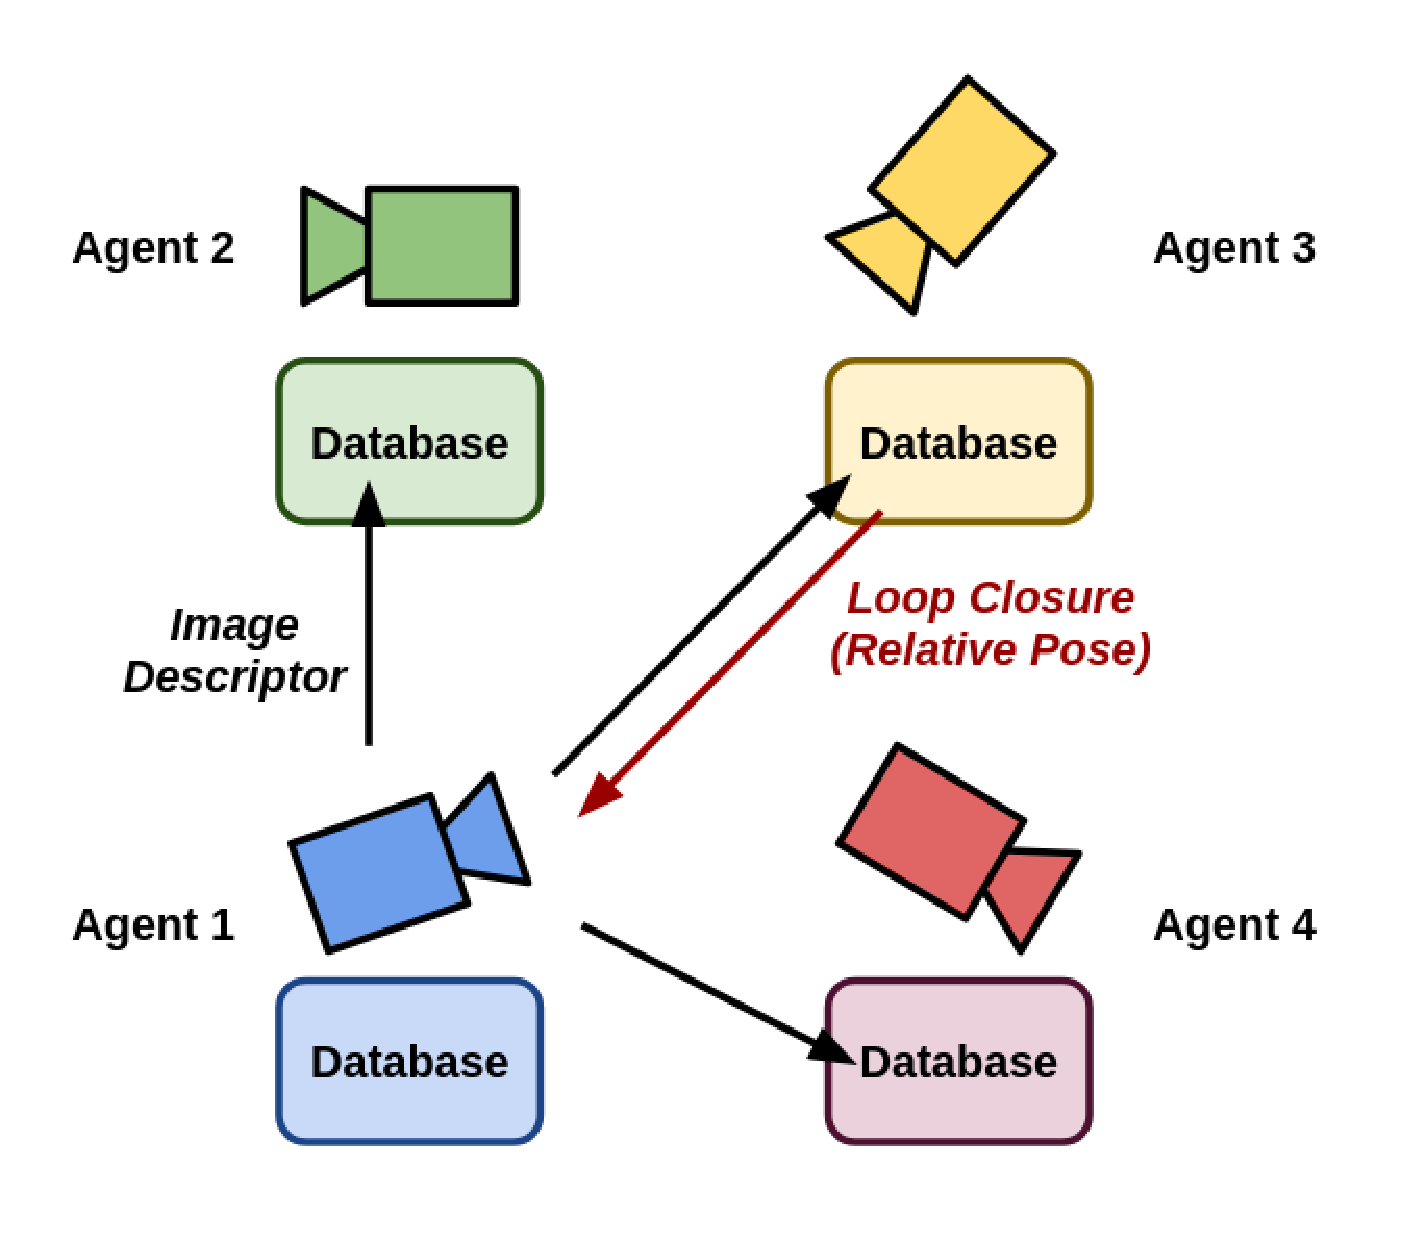
\includegraphics[width=\linewidth]{Fig/simple_model.eps}
		\caption{Model of Collaborative Visual Inertial System. During communication, agent1 sends image feature data to agent3, and agent3 matches this data with its own database. When a match is detected, agent3 sends relative position data to agent1 via the communication edge.}
		\label{fig:simple_model}
	\end{center}
	\vspace{-2mm}
\end{figure}

\subsection{Related Work}
This research is related to the fields of Visual Inertial Systems (VINS), multi-robot collaborative SLAM, and particle filters and variational inference.

VINS is a method that combines cameras and IMUs for self-localization and is widely used in environments where GPS/GNSS is unavailable. Qin et al. \cite{Qin2018} proposed VINS-Mono, a robust and versatile VINS using a monocular camera and IMU, integrating features such as feature point tracking, IMU pre-integration, and loop detection. Bloesch et al. \cite{Bloesch2017} proposed an extended Kalman filter-based VINS using direct photometric feedback, achieving a method independent of feature point extraction. Forster et al. \cite{Forster2017} proposed a real-time VINS using pre-integration on manifolds, demonstrating an efficient method for processing IMU measurements. These studies focus on single agents and do not adequately address the challenges of multiple agents' collaboration or monotone environments.

Multi-robot collaborative SLAM is a method where multiple robots cooperate to map the environment and estimate their positions. Chen et al. \cite{Chen2021} summarized multi-robot collaborative SLAM from a data fusion perspective, classifying and comparing various approaches such as centralized, distributed, and decentralized. Zhou et al. \cite{Zhou2018} conducted research on swarms of micro aerial robots in actual outdoor environments, demonstrating challenges and solutions for collaborative self-localization. Xu et al. \cite{Xu2020} proposed D2SLAM, a distributed collaborative Visual-Inertial SLAM system, achieving efficient collaborative self-localization for aerial swarms. These studies focus on the collaboration of multiple agents but do not adequately address robustness to outliers in monotone environments or the handling of multi-modal distributions.

Particle filters and variational inference are methods for solving non-Gaussian and non-linear probabilistic state estimation problems. Liu and Wang \cite{Liu2016} proposed Stein Variational Gradient Descent (SVGD), a general Bayesian inference algorithm that forms the basis of the SPF used in this research. Maken et al. \cite{Maken2021} proposed SPF for non-linear and non-Gaussian state estimation, solving the problem of particle degradation due to resampling in conventional particle filters. Koide et al. \cite{Koide2021} conducted research on accelerating SPF using GPUs, achieving real-time 6-degree-of-freedom position estimation. These studies focus on the theory and application of particle filters and variational inference but do not adequately address the combination with multiple agent collaboration or consensus problems.

\subsection{Contributions}

The main contributions of this research are as follows:
\begin{itemize}
\item We formulated SPF for multi-agents in the special Euclidean space to handle 2D and 3D cooperative self-localization uniformly. This enables application to practical cooperative self-localization requiring 3D estimation, such as visual inertial systems.
\item We proposed an SPF algorithm that enables global (consistent across multiple agents) convergence through the introduction of ADMM. This achieves consistent state estimation among agents, which was difficult with conventional distributed cooperative estimation methods.
\item By acquiring ambiguity representation in cooperative self-localization, we proposed an estimation method robust to outliers, which has been a fundamental problem in monotone environments. Specifically, by combining the particle-based method with representation capability for multi-modal distributions and Stein Variational Gradient Descent utilizing gradient information, we localized the influence of outliers and improved the overall system estimation accuracy.
\end{itemize}

\section{Preliminary}

\subsection{Stein Variational Gradient Descent}
Consider the following Kullback-Leibler divergence minimization problem:

\begin{equation}
\begin{aligned}\label{eq:kl_min}
 q^{*}&=\underset{q \in \mathcal{Q}}{\text{arg min}}\left\{D_{KL}(q \| p) \equiv {{\mathbb{E}}}_{q}[\log q(x)]-{{\mathbb{E}}}_{q}[\log {p}(x)] \right\},
\end{aligned}
\end{equation}

The following theorem holds:

\begin{theorem}[Relationship between KL Divergence and Stein Operator]
For a transformation ${\boldsymbol{T}}(x)=x+\epsilon {\boldsymbol{\Phi}}(x)$, where $x \sim q(x)$ and the probability distribution of $z={\boldsymbol{T}}(x)$ is denoted as $q_{[{\boldsymbol{T}}]}(z)$,
\begin{equation}
\begin{aligned}\label{eq:kl_gradient}
\left.\nabla_{\epsilon} D_{KL}\left(q_{[{\boldsymbol{T}}]} \| p\right)\right|_{\epsilon=0}=-{{\mathbb{E}}}_{x \sim q}\left[{\mathcal{A}}_{p} {\boldsymbol{\Phi}}(x)\right],
\end{aligned}
\end{equation}
holds, where ${\mathcal{A}}_{p} {\boldsymbol{\Phi}}(x)=\nabla_{x} \log p(x) {\boldsymbol{\Phi}}(x)^{\top}+\nabla_{x} {\boldsymbol{\Phi}}(x)$ is the Stein Operator, and ${\boldsymbol{\Phi}}$ is a functional belonging to the reproducing kernel Hilbert space ${\mathcal{H}}^d$.
\end{theorem}

Defining the Kernelized Stein Discrepancy (KSD) as

\begin{equation}
\begin{aligned}\label{eq:ksd}
{{\mathbb{D}}}(q,p)&=\max_{{\boldsymbol{\Phi}}\in {\mathcal{H}}^d}{{\mathbb{E}}}_{x \sim q}\left[{\mathcal{A}}_{p} {\boldsymbol{\Phi}}(x)\right], 
\quad \text{s.t.} \quad \|{\boldsymbol{\Phi}}\|_{{\mathcal{H}}^d} \leq 1,
\end{aligned}
\end{equation}

the solution to this problem is given by

\begin{equation}
\begin{aligned}\label{eq:phi_solution}
{\boldsymbol{\Phi}}_{q, p}^{*}(\cdot)={{\mathbb{E}}}_{x \sim q}\left[k(x, \cdot) \nabla_{x} \log p(x)+\nabla_{x} k(x, \cdot)\right],
\end{aligned}
\end{equation}

\subsection{Relaxed ADMM}

The following constrained optimization problem with two variables

\begin{equation}
\begin{aligned}\label{eq:constrained_opt}
&\min_{x,y} f(x)+g(y), \quad \text{s.t.}\: Ax+By=b,
\end{aligned}
\end{equation}

can be solved using the following augmented Lagrangian

\begin{equation}
\begin{aligned}\label{eq:augmented_lagrangian}
{\mathcal{ L}}_{f,\gamma}(z) &= f(x) - \langle z, Ax \rangle + \frac \gamma 2 \|Ax\|^2,\\
{\mathcal{ L}}_{g,\gamma}(z) &=  g(y) - \langle z, By-b \rangle + \frac \gamma 2 \|By-b\|^2,
\end{aligned}
\end{equation}

with the dual ascent method as follows \cite{Peng2016}\cite{Boyd2011}:

\begin{equation}
\begin{aligned}\label{eq:relaxed_admm_steps}
y^+&= \underset{y}{\text{arg min}}\: {\mathcal{ L}}_{g,\gamma}(z),\\
\omega_g &=  z - \gamma (By^+-b), \\
x^+&= \underset{x}{\text{arg min}}\: {\mathcal{ L}}_{f,\gamma}(2\omega_g - z),\\
\omega_f &= 2\omega_g - z - \gamma Ax^+,\\
z^+&=z+\eta(\omega_f-\omega_g),
\end{aligned}
\end{equation}

\section{Problem Formulation}

In this paper, we address cooperative self-localization of agents in Euclidean space ${{\mathbb{R}}}^d$.
The state of agent $i$ at time step $t$ is denoted as $x_i^t=({\mathbf{t}}^t_i, R^t_i)\in \mathrm{SE}(d):={{\mathbb{R}}}^d\times \mathrm{SO}(d)$, where ${\mathbf{p}}^t_i\in{{\mathbb{R}}}^d$ is the coordinate and $R^t_i\in \mathrm{SO}(d)$ is the rotation matrix. In our method validation, we conduct tests for cases where $d=2$ and $d=3$. Cooperative self-localization, with observations from each agent denoted as $z^t=[z_1^t, \cdots, z_N^t]$, can be formulated as the following maximum a posteriori estimation problem (MAP estimation problem):

\begin{equation}
\begin{aligned}\label{eq:map}
\underset{x^{t+1}_1, \cdots, x^{t+1}_N}{\text{max}} \: \sum^N_{i=1} P(x^{t+1}_i|Z_i^{t}) Q(z_i^{t+1}|x_i^{t+1}),
\end{aligned}
\end{equation}

where the distribution $P(x^{t+1}_i|Z_i^{t})$ represents the probability distribution of agent $i$'s state at time step $t+1$ before the observation information $z_i^{t+1}$ is given, and the distribution $Q(z_i^{t+1}|x_i^{t+1})$ represents the likelihood distribution of obtaining observation information $z_i^{t+1}$ at state $x_i^{t+1}$. Here, $Z_i^t = [z_i^0 \cdots z_i^t]$.

The 3D special Euclidean group $\mathrm{SE(3)}$ is represented in the following form:

\begin{equation}
\begin{aligned}\label{eq:se3_matrix}
T = 
\begin{pmatrix}
{\mathbf{R}} & {\mathbf{t}} \\
{\mathbf{0}}^T & 1
\end{pmatrix}
=
\begin{pmatrix}
{\mathbf{d}}_{c1} & {\mathbf{d}}_{c2} & {\mathbf{d}}_{c3} & {\mathbf{t}} \\
0 & 0 & 0 & 1
\end{pmatrix} \in {{\mathbb{R}}}^{4\times4},
\end{aligned}
\end{equation}

We introduce the following operators for the special orthogonal group $\mathrm{SO(d)}$ and the special Euclidean group $\mathrm{SE(d)}$:

\begin{equation}
\begin{aligned}
(\cdot)^{\wedge}&: {{\mathbb{R}}}^{\frac{d(d-1)}{2}} \rightarrow  {\mathfrak{so}}(d), {{\mathbb{R}}}^{d+\frac{d(d-1)}{2}} \rightarrow  {\mathfrak{se}}(d),\\
{\boldsymbol{\omega}}&=\begin{bmatrix}
    \:x\: \\
    \:y\: \\
    \:z\: 
\end{bmatrix}\in{{\mathbb{R}}}^3,
\quad {\boldsymbol{\omega}}^{\wedge}=\begin{pmatrix}
    0&-z&y \\
    z&0&x \\
    -y&x&0 
\end{pmatrix}\in {\mathfrak{so}}(3)\\
{\mathbf{v}}&=\begin{bmatrix}
    \:{\mathbf{t}}\: \\
    \:{\boldsymbol{\omega}}\: 
\end{bmatrix}\in{{\mathbb{R}}}^6,\quad {\mathbf{v}}^\wedge=\begin{pmatrix}
    {{\boldsymbol{\omega}}^\wedge}& {\mathbf{t}}\\
    0&1
\end{pmatrix}\in {\mathfrak{se}}(3)
\end{aligned}
\end{equation}

\begin{equation}
\begin{aligned}
\exp&:  {\mathfrak{so}}(d) \rightarrow  \text{SO}(d),{\mathfrak{se}}(d) \rightarrow  \text{SE}(d),\\
\quad e^{{\boldsymbol{\omega}}} &\equiv \exp({{\boldsymbol{\omega}}}^\wedge) \\
&= {\mathbf{I}}_3 + \frac{\sin \theta}{\theta } {{\boldsymbol{\omega}}}^\wedge+\frac{1-\cos \theta }{\theta^2}({{\boldsymbol{\omega}}}^\wedge)^2 \in \text{SO}(3)\\
e^{{\mathbf{v}}}&\equiv \exp({{\mathbf{v}}^\wedge}) = 
\begin{pmatrix}
    e^{{{\boldsymbol{\omega}}}^\wedge}& {\mathbf{V}}{\mathbf{t}}\\
    0&1
\end{pmatrix}\in\text{SE}(3),\quad \\
{\mathbf{V}}&={\mathbf{I}}_3+\frac{1-\cos\theta}{\theta^2}{{\boldsymbol{\omega}}}^\wedge +\frac{\theta-\sin \theta}{\theta^3}({{\boldsymbol{\omega}}}^\wedge)^2
\end{aligned}
\end{equation}

Additionally, $()^\vee$ and $\log$ represent the inverse operations of $()^\wedge$ and $\exp$, respectively.
As a common approach in SPF, equation (\ref{eq:map}) can be rewritten as a Kullback-Leibler divergence (KL divergence) $D_{KL}$ minimization problem:

\begin{equation}
\begin{aligned}
  &\underset{x_i^{t+1}}{\text{max}} \:  P(x_i^{t+1}|Z_i^{t}) Q(z_i^{t+1}|x_i^{t+1})\\
  &\simeq \underset{x_i^{t+1}}{\text{max}} \: \underset{P_{[T]}}{\text{arg min}} \: D_{KL}(P(x_i^{t+1}|Z_i^{t})_{[T]} \| P_Q),
\end{aligned}
\end{equation}

where the target distribution $P_Q$ is a probability distribution of state $x_i^{t+1}$ isomorphic to the likelihood distribution $Q$, and can be represented as a superposition of kernels on $\mathrm{SE(3)}$ using mean coordinate $\mu\in\mathrm{SE}(d)$ and weight diagonal matrix $\Sigma \in {{\mathbb{R}}}^{(d+\frac{d(d-1)}{2})\times (d+\frac{d(d-1)}{d})}$:

\begin{equation}
\begin{aligned}
{\mathcal{K}}_j&=\exp \left(-(d_j^\vee)^{\top} \Sigma d_j^\vee \right)\in {{\mathbb{R}}},\\
d_j&=\log \left((\mu_j^{-1}) x_i^{t+1} \right)\in {\mathfrak{se}}(d)
\end{aligned}
\end{equation}

From these backgrounds, by defining the state of agent $j$ as seen from agent $i$ at time step $t$ as $x_{i,j}^t$ and modifying the state to be estimated as $\hat x_i^t= \left\{ x_{i,j}^t \in \mathrm{SE(d)}\: | \: j \in \mathcal{N}_i \right\}$, the problem to be solved can be formulated as:
\begin{equation}
\begin{aligned}\label{eq:kl_consensus}
\max _{\hat x_{1}^{t}, \cdots, \hat x_{N}^{t}} & \sum_{i=1}^{N} \arg \min _{{P_{i}}_{[T]}} D_{K L}\left(P_{i}\left(\hat x_{i}^{t} \mid Z_{i}^{t-1}\right)_{\left[T_{i}]\right.} \| P_{Q_{i}} \right) \\
\text { s.t. } & \hat x_{i}^{t}=\hat x_{j}^{t}, \quad\forall(i, j) \in \mathcal{E}
\end{aligned}
\end{equation}
The constraint in equation (\ref{eq:kl_consensus}) indicates that the estimated states of drones must match across all edges $\mathcal{E}$ representing communication between agents.

\section{SPF For Collaborative Localization}

In this section, we propose a mathematical algorithm using SPF to solve equation (\ref{eq:kl_consensus}). While the minimization of KL divergence in probability distributions can be numerically calculated using SPF, minimizing KL divergence in multi-agent problems is very challenging because there is no target distribution fixed to absolute coordinates, and the target distribution $P_{Q_i}$ itself becomes a dependent variable of the state to be estimated. Furthermore, if a straightforward SPF algorithm without constraints like equation (\ref{eq:kl_consensus}) is applied, the filtering algorithm is optimized only for partial state quantities, and as discussed later, it cannot create a unified relative position graph for all agents, causing estimation to fail. To solve these problems, we formulated an SPF algorithm applicable to Collaborative Localization using explicit likelihood functions based on relative positions between particles and a consensus algorithm using Relaxed ADMM.

\subsection{Gradient Effect Between Particles}

First, we approximate the probability distribution as $P_{i}\left( x_{i}^{t} \mid Z_{i}^{t-1}\right)\simeq \left\{ p_{i,l}\in \mathrm{SE(3)} \right\}_{l=1:m}$ using particles, and consider gradient descent of these particles along the target distribution $P_{Q_i}$ based on equation (\ref{eq:kl_consensus}).

\begin{equation}
\begin{aligned}\label{eq:svgd_min}
&\underset{P_{[T]}}{\text{min}} \: \nabla_\epsilon \left . D_{KL}(P(x_i^{t+1}|Z^{t})_{[T]} \| P_{Q_i})\right |_{\epsilon = 0},\\
&\Rightarrow p_{i,l}:= p_{i,l} \exp({\boldsymbol{\Phi}}^*),\\
&\quad \:\: {\boldsymbol{\Phi}}^*(p_{i,l}) = \frac{1}{m}\sum_{r=1}^m(\nabla_{p_{i,r}}\log P_Q(p_{i,r})k(p_{i,l},p_{i,r}) \\
&\qquad \qquad \quad \: + \nabla_{p_{i,j}}k(p_{i,l},p_{i,r})),
\end{aligned}
\end{equation}
where $k(p_{i,l},p_{i,r})=\exp \left(-(d_j^\vee)^{\top} \Sigma d_j^\vee \right)\in \mathbb{R}$ is a kernel on $\mathrm{SE(3)}$.

\begin{equation}
\begin{aligned}\label{eq:log_target_dist}
    \log P_{Q_i}(p_{i,r}) &= \log \prod_{k\in {\mathcal{N}}} {\mathcal{K}}_k\\
    &= -\sum_{k\in {\mathcal{N}}} (d_k^\vee)^{\top} \Sigma_k d_k^\vee \in \mathbb{R},\\
d_k(p_{i,r})&=\log \left(p_{j,k}^{-1} (p_{i,r}T_{i\rightarrow j}) \right)\in {\mathfrak{se}}(d)
\end{aligned}
\end{equation}

where $k\in{\mathcal{N}} := {\mathcal{N}}_{j}(p_{i,l}T_{i\rightarrow j})$ represents the set of particles in the neighborhood of the $r$-th particle of agent $i$, $p_{i,r}$, transformed by $T_{i\rightarrow j}\in \mathrm{SE(3)}$, among the particles held by agent $j$. By explicitly calculating the error on $\mathrm{SE(3)}$ for particles in the neighborhood of the predicted position transformed along the obtained relative position $T_{i\rightarrow j}$, and estimating the true target distribution in the neighborhood using KDE, it is possible to minimize KL divergence even when there is no fixed target distribution.
To further accelerate convergence, the gradient of the target distribution $\nabla_{p_{i,r}}\log P_Q(p_{i,r})$ is calculated using the Gauss-Newton method:
\begin{equation}
% \begin{equation}
\begin{aligned}\label{eq:gauss_newton}
\nabla_{p_{i,r}}\log P_Q(p_{i,r})&:=
({\mathbf{H}}^r)^{-1}b^r,\\
{\mathbf{H}}^r &= ({\mathbf{J}}^r)^\top {\mathbf{J}}^r, \\
b^r&=({\mathbf{J}}^r)^\top d_k(p_{i,r})^\vee,\\
{\mathbf{J}}^r&=\left. \frac{\partial(d_k(p_{i,r}e^{{{\boldsymbol{\varepsilon}}}})^\vee
)}{\partial {{\boldsymbol{\varepsilon}}}}\right|_{{{\boldsymbol{\varepsilon}}}={\mathbf{0}}}
\end{aligned}
% \end{equation}
\end{equation}

\subsection{SPF integrating Relaxed ADMM}

In this subsection, we formulate an algorithm to minimize KL divergence with consensus constraints as in equation (\ref{eq:kl_consensus}), based on the gradient descent method using SPF formulated in subsection A. First, as a straightforward solution, consider:
\begin{equation}
\begin{aligned}
&\underset{P_{[T]}}{\text{min}} \: \nabla_\epsilon \left . D_{KL}(P(x_i^{t+1}|Z^{t})_{[T]} \| P_{Q_i})\right |_{\epsilon = 0}, \quad 
\forall i\in \mathcal{A}
\end{aligned}
\end{equation}
where all agents update their relative position particles at the point when they receive relative positions for each agent pair. In this case, since there is no guarantee that the source agent of the relative position has converged to a globally correct position, as shown in Fig. \ref{fig:parallel_update}(a), optimization occurs only for specific agent pairs, making it impossible to construct a consistent relative position graph for all agents. Various optimizations through filtering can only optimize a single state quantity partially, not multiple state quantities simultaneously. Here, we formulate an algorithm that enables global convergence regardless of the order in which relative positions are obtained, using a consensus filter with ADMM as shown in Fig. \ref{fig:parallel_update}(b).

\begin{figure}[t]
	\begin{center}
		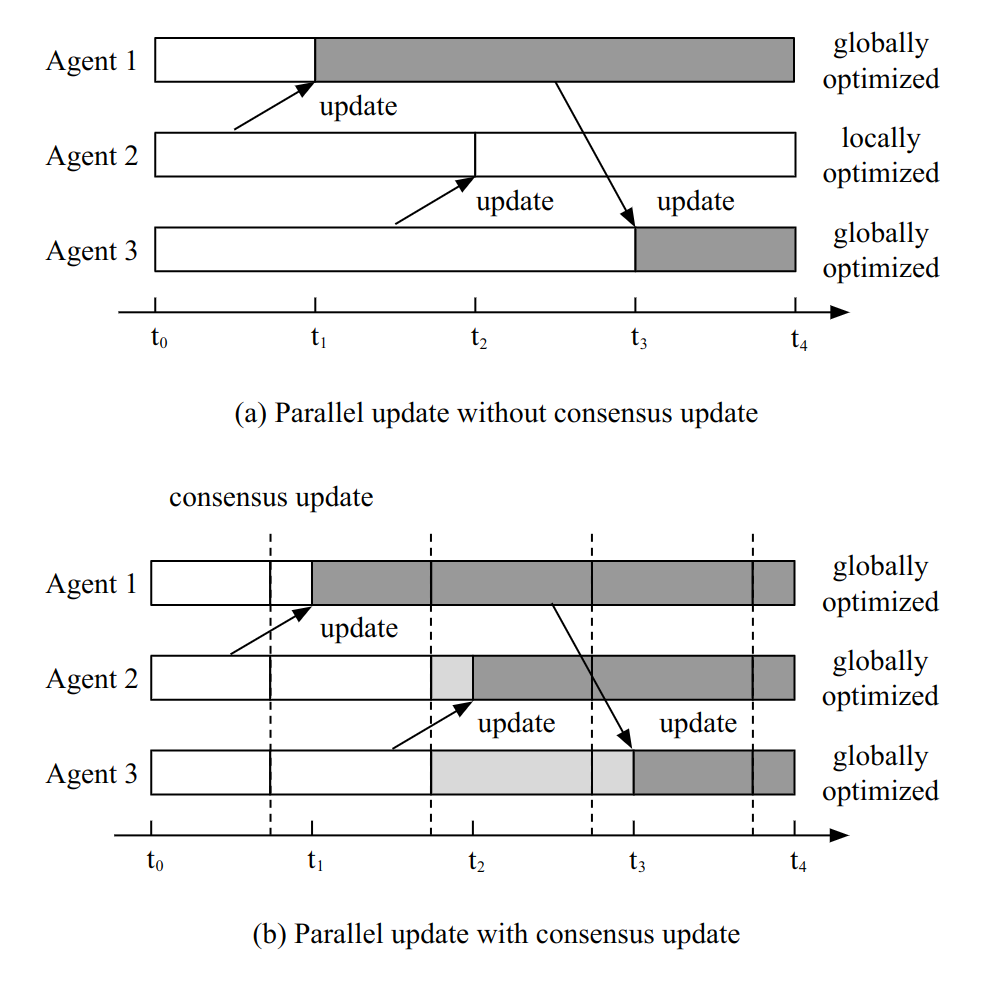
\includegraphics[width=\linewidth]{Fig/parallel_update1.eps}
		\caption{Sequence diagram of each agent receiving relative positions and updating estimated states in parallel in a system like Fig. \ref{fig:simple_model}. (a) shows a straightforward method without consensus rules, (b) shows a method enabling global convergence using consensus rules.}
		\label{fig:parallel_update}
	\end{center}
	\vspace{-2mm}
\end{figure}

Equation (\ref{eq:kl_consensus}) can be relaxed using slack variables $y_{i,j}$ as:
\begin{equation}
\begin{aligned}
\max _{\hat x_{1}^{t}, \cdots, \hat x_{N}^{t}} & \sum_{i=1}^{N} \arg \min _{{P_{i}}_{[T]}} D_{K L}\left(P_{i}\left(\hat x_{i}^{t} \mid Z_{i}^{t-1}\right)_{\left[T_{i}]\right.} \| P_{Q_{i}} \right) \\
\text { s.t. } & \hat x_{i}^{t}=y_{i,j}, \:\hat x_{j}^{t}=y_{i,j}, \quad\forall(i, j) \in \mathcal{E}
\label{eq:kl_consensus_relaxed}
\end{aligned}
\end{equation}
which reduces to the problem in equation (7).

\begin{definition}[Augmented Lagrangian for Probability Distributions]
We redefine the augmented Lagrangian for Relaxed ADMM, taking probability distributions as arguments, as:
\begin{equation}
\begin{aligned}
 {\mathcal{ L}}_{F,\gamma}(x_i, \zeta) 
 = F_i(x_i) - \int_{{\mathcal{X}}_i}
\zeta dx_i + \frac{\gamma}{2}\int_{{\mathcal{X}}_i} dx_i^2,
\label{eq:relaxed_lagrangian}
\end{aligned}
\end{equation}
\end{definition}

The following theorem presents the Relaxed ADMM algorithm for probability distributions to solve equation (\ref{eq:kl_consensus_relaxed}).

\begin{theorem}[Relaxed ADMM Algorithm for Probability Distributions]
The constrained optimization problem for probability distributions represented by equation (\ref{eq:kl_consensus_relaxed}) can be solved using the following Relaxed ADMM algorithm:
\begin{equation}
\begin{aligned}
x^+_i&= \underset{x_i}{\text{arg min}}\: D_{KL} ({P_i}_{[T]}\|{P_Q}_i) \\
&+ \sum_{r\in {\mathcal{E}}_i} \int_{P_i}  z_{ir,r} dx_i + \frac{\gamma}{2}|{\mathcal{E}}_i|\int_{P_i} dx_i^2,\\
&= \underset{x_i}{\text{arg min}}\: D_{KL} ({P_i}_{[T]}\|{P_Q}_i) \\
&+ \frac{\gamma}{2} \:{\mathbb{E}}_{x_i\sim P_i}\left[\sum_{\gamma \in {\mathcal{E}}_i} \|x_i + z^+_{ir,i}/\gamma \|^2\right],\\
z^+_{ir,i} &=z_{ir,i}+\eta((z_{ir,i} + z_{ir,r})/2 + \gamma x_{i}).\quad  \forall r \in {\mathcal{E}}_i,
\label{eq:prob_relaxed_admm}
\end{aligned}
\end{equation}
where $x^+_i$ is the updated state, $z_{ir,i}$ are Lagrange multipliers, $\gamma$ is the penalty parameter, and $\eta$ is the step size parameter. This algorithm simultaneously optimizes both the local probability distributions of each agent and the consensus constraints between agents.
\end{theorem}

This algorithm enables simultaneous optimization of consensus constraints among multiple agents and probability distributions, achieving stable state estimation even in environments with outliers.

\begin{theorem}[Additional Terms as Exponential Penalties]
Consider the following optimization problem:
\begin{equation}
\begin{aligned}
&\min_{P_i}  D_{KL}(P_i \,\|\, P_{Q_i}) \\
&+ \sum_{r \in {\mathcal{E}}_i} \int P_i(x_i) z_{ir,r}(x_i)\,dx_i 
+ \frac{\gamma}{2}|{\mathcal{E}}_i| \int P_i(x_i) x_i^2\, dx_i
\end{aligned}
\end{equation}
where $\int P_i(x_i)dx_i=1$ and $D_{KL}(P_i \,\|\, P_{Q_i})$ is defined as:
\begin{equation}
\begin{aligned}
&\underset{x_i^{t+1}}{\text{max}} \:  P(x_i^{t+1}|Z_i^{t}) Q(z_i^{t+1}|x_i^{t+1})\\
&\simeq \underset{x_i^{t+1}}{\text{max}} \: \underset{P_{[T]}}{\text{arg min}} \: D_{KL}(P(x_i^{t+1}|Z_i^{t})_{[T]} \| P_Q),
\end{aligned}
\end{equation}
The optimal distribution $P_i^*$ for this optimization problem can be expressed using a normalization constant $Z$ as:
\begin{equation}
\begin{aligned}
P_i^*(x_i) = \frac{P_{Q_i}(x_i)\exp\left(- \sum_{r \in {\mathcal{E}}_i} z_{ir,r}(x_i) 
- \frac{\gamma}{2}|{\mathcal{E}}_i| x_i^2\right)}{Z},
\end{aligned}
\end{equation}
Thus, the additional penalty terms:
\begin{equation}
\begin{aligned}
\sum_{r \in {\mathcal{E}}_i} z_{ir,r}(x_i) \;+\; \frac{\gamma}{2}|{\mathcal{E}}_i|x_i^2,
\end{aligned}
\end{equation}
characterize the optimal solution by applying exponential weights (penalties) to the reference distribution $P_{Q_i}(x_i)$.
\end{theorem}

Therefore, from equation (\ref{eq:prob_relaxed_admm}), the particle update rule can be modified as:
\begin{equation}
\begin{aligned}
&\underset{x_i}{\text{min}}\: D_{KL} ({P_i}_{[T]}\|{P_Q}_i) \\
&\quad \:\: + \sum_{r\in {\mathcal{E}}_i} \int_{P_i} z_{ir,r} dx_i + \frac{\gamma}{2}|{\mathcal{E}}_i|\int_{P_i} dx_i^2,\\
&\Rightarrow p_{i,l}:= p_{i,l} \exp({\boldsymbol{\Phi}}^*),\\
&\quad \:\: {\boldsymbol{\Phi}}^*(p_{i,l}) = \frac{1}{m}\sum_{r=1}^m(\nabla_{p_{i,r}}\log {{P}^*_i}(p_{i,r})k(p_{i,l},p_{i,r}) \\
&\qquad \qquad \quad \: + \nabla_{p_{i,j}}k(p_{i,l},p_{i,r})),\\
&\quad \:\:  {{P}^*_i}(p_{i,r}) \propto {P}_{Q_i}(p_{i,r})\exp\left(- \sum_{r \in  {\mathcal{E}}_i} z_{ir,r}(p_{i,l}) - \frac{\gamma}{2}|{\mathcal{E}}_i| p_{i,l}^2\right),
\label{eq:modified_SVGD}
\end{aligned} 
\end{equation}

With these formulations, the algorithm to solve equation (\ref{eq:map}) can be expressed as follows:

\begin{algorithm}[h]
\caption{SPF For Collaborative Localization}\label{alg:dspf}

\begin{algorithmic}[1]
\STATE \textbf{Input:} $n$ UAVs, $m$ particles $\{x^t_{i,j}\}^m_{j=1}$, Target distribution ${P_Q}_i$

\FOR{$k = 1$ to $K$}
\STATE preintegration by (\ref{eq:predict})
\ENDFOR
\STATE $\forall_{j=1:m}\; p^{t+1}_{i,j} = p^{t}_{i,j} T^{t \rightarrow {t+1}}$  // prediction (\ref{eq:step})
\FOR{$l = 1$ to $L$}
\STATE $\forall_{j=1:m}\;$ update particle by (\ref{eq:modified_SVGD})
\STATE $x_i = \underset{x_i}{\text{arg min}}\: {P_i(x_i)}$ // local MAP estimation
\STATE consensus update by (\ref{eq:prob_relaxed_admm})
\ENDFOR
\end{algorithmic}
\end{algorithm}

\section{Simulation Result with Collaborative Localization}

Based on the proposed algorithm, we conducted simulations of cooperative self-localization in both 2D and 3D cases. In the algorithm implementation, to reduce computational load, all algorithms were implemented on CUDA, and particle updates were processed in parallel on the GPU. cuSolver was used for solving the Gauss-Newton method. The hardware used was a PC equipped with an Intel Core Ultra 9 and NVIDIA GeForce RTX 4060.

\subsection{Two-dimensional case}

As a validation of the proposed method, we conducted a simulation of a 2D cooperative self-localization scenario. The simulation conditions are shown in Table \ref{tb:sim1}.

\begin{table}[h]
\caption{Simulation Conditions}
  \centering
  \begin{tabular}{l|c} \hline
    Item & Value  \\ \hline
    Number of agents & 3  \\
    Number of particles per agent & 50  \\ 
    Number of time steps & 250 \\
    Total number of matches & 250 \\ 
    Number of incorrect matches & 52 \\
    Proportion of outliers & $\simeq$ 0.2 \\ \hline
  \end{tabular}
  \label{tb:sim1}
\end{table}

In the simulation, we assumed that the relative positions between random agent pairs (pseudo loop closures, black dotted lines in Fig. \ref{fig:simulation_1_step_0}) are obtained at each step, and used this relative information to estimate the position of each agent.
We also assumed that incorrect relative positions (red dotted lines in Fig. \ref{fig:simulation_1_step_0}) are obtained with a proportion of about 0.2, and conducted a cooperative self-localization simulation using matplotlib.
Fig. \ref{fig:simulation_1_step_0}(a) left shows the true positions of each agent, and Fig. \ref{fig:simulation_1_step_0}(a) right shows the estimation screen.
Incorrect relative positions were generated from random coordinates within the simulation area and the true positions of each agent.

Fig. \ref{fig:simulation_1_step_0}(a) and (b) show the estimated states of each agent at 0 steps and 150 steps, respectively.
From these, it can be seen that the probability distributions (particles) that were initially uniformly set have converged to reasonable positions at 150 steps.
Fig. \ref{fig:plot_1} shows the time transition of the coordinates of all particles in the simulation.
From Fig. \ref{fig:plot_1}, it can also be seen that consensus and convergence are achieved after about 150 steps.

\begin{figure}[t]
	\begin{center}
		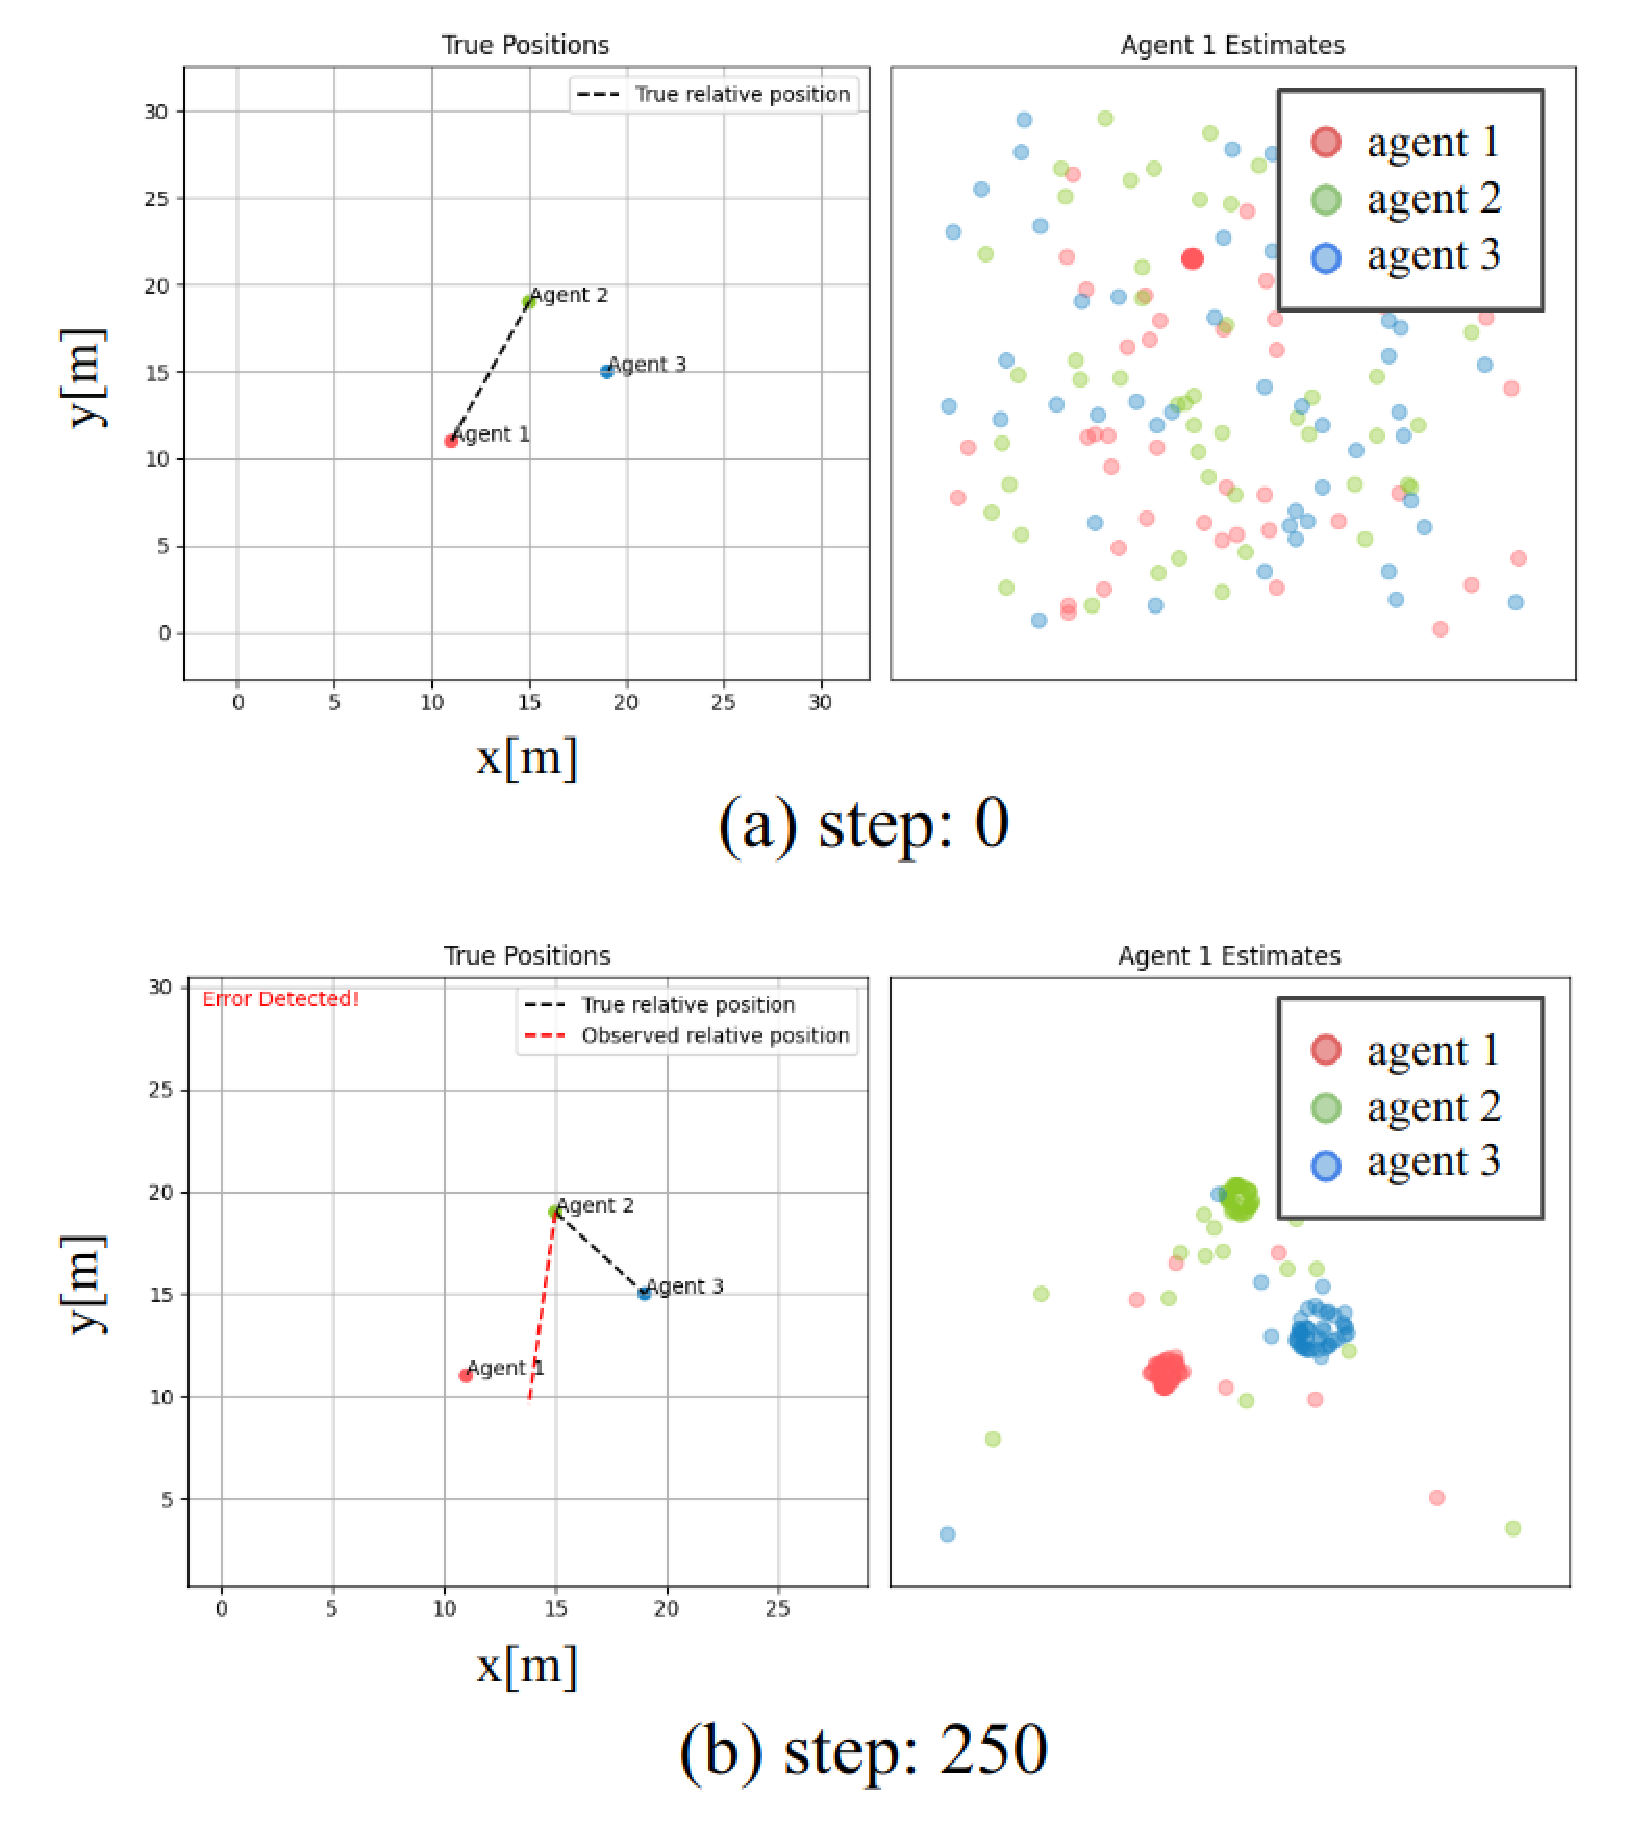
\includegraphics[width=\linewidth]{Fig/2d_simulation.eps}
		\caption{Two-dimensional cooperative self-localization simulation with an outlier ratio of 0.2. (a) shows the initial state, (b) shows the state at 150 steps.
    The left figure shows the true positions of each agent, and the points in the right figure are the coordinates $p_{i,r}$ of the particles for each agent.}
		\label{fig:simulation_1_step_0}
	\end{center}
	\vspace{-2mm}
\end{figure}

% \begin{figure}[t]
% 	\begin{center}
% 		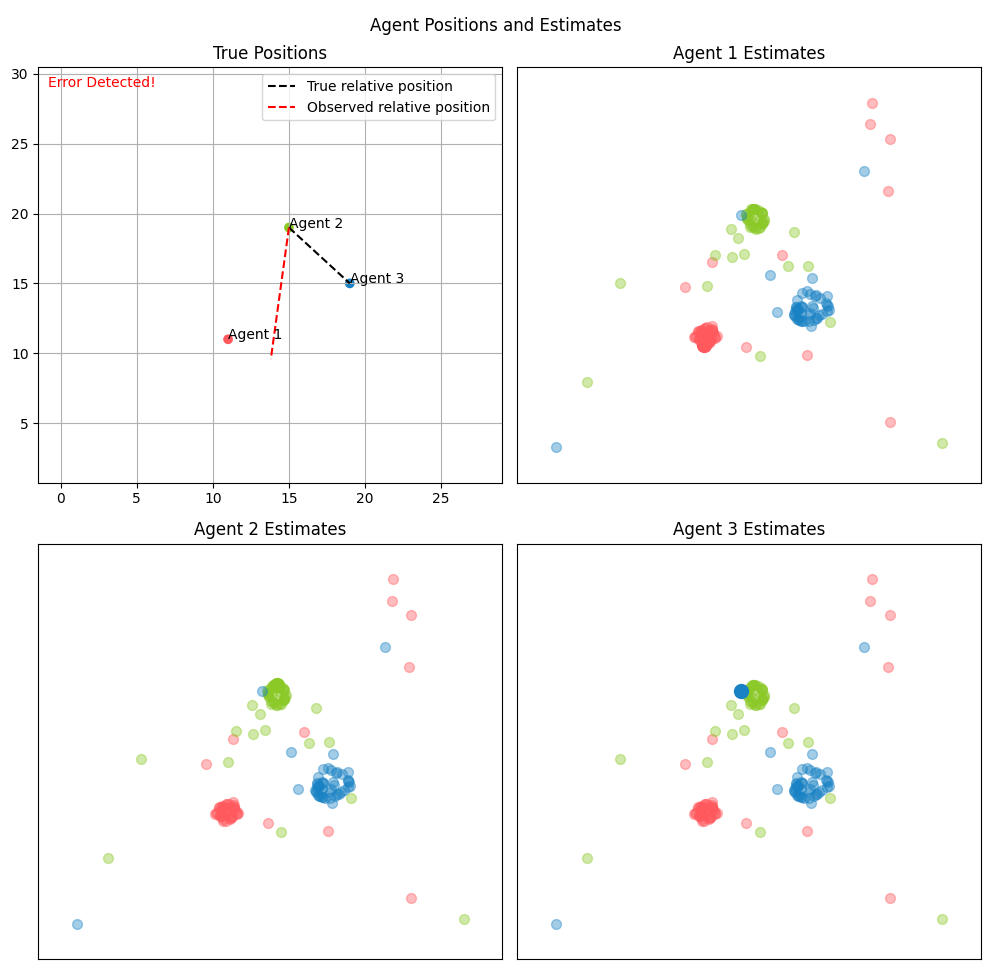
\includegraphics[width=\linewidth]{Fig/error_0.2_sim.eps}
% 		\caption{Simulation (Outlier ratio: 0.2, step: 150)}
% 		\label{fig:simulation_1_step_150}
% 	\end{center}
% 	\vspace{-2mm}
% \end{figure}

\begin{figure}[t]
	\begin{center}
		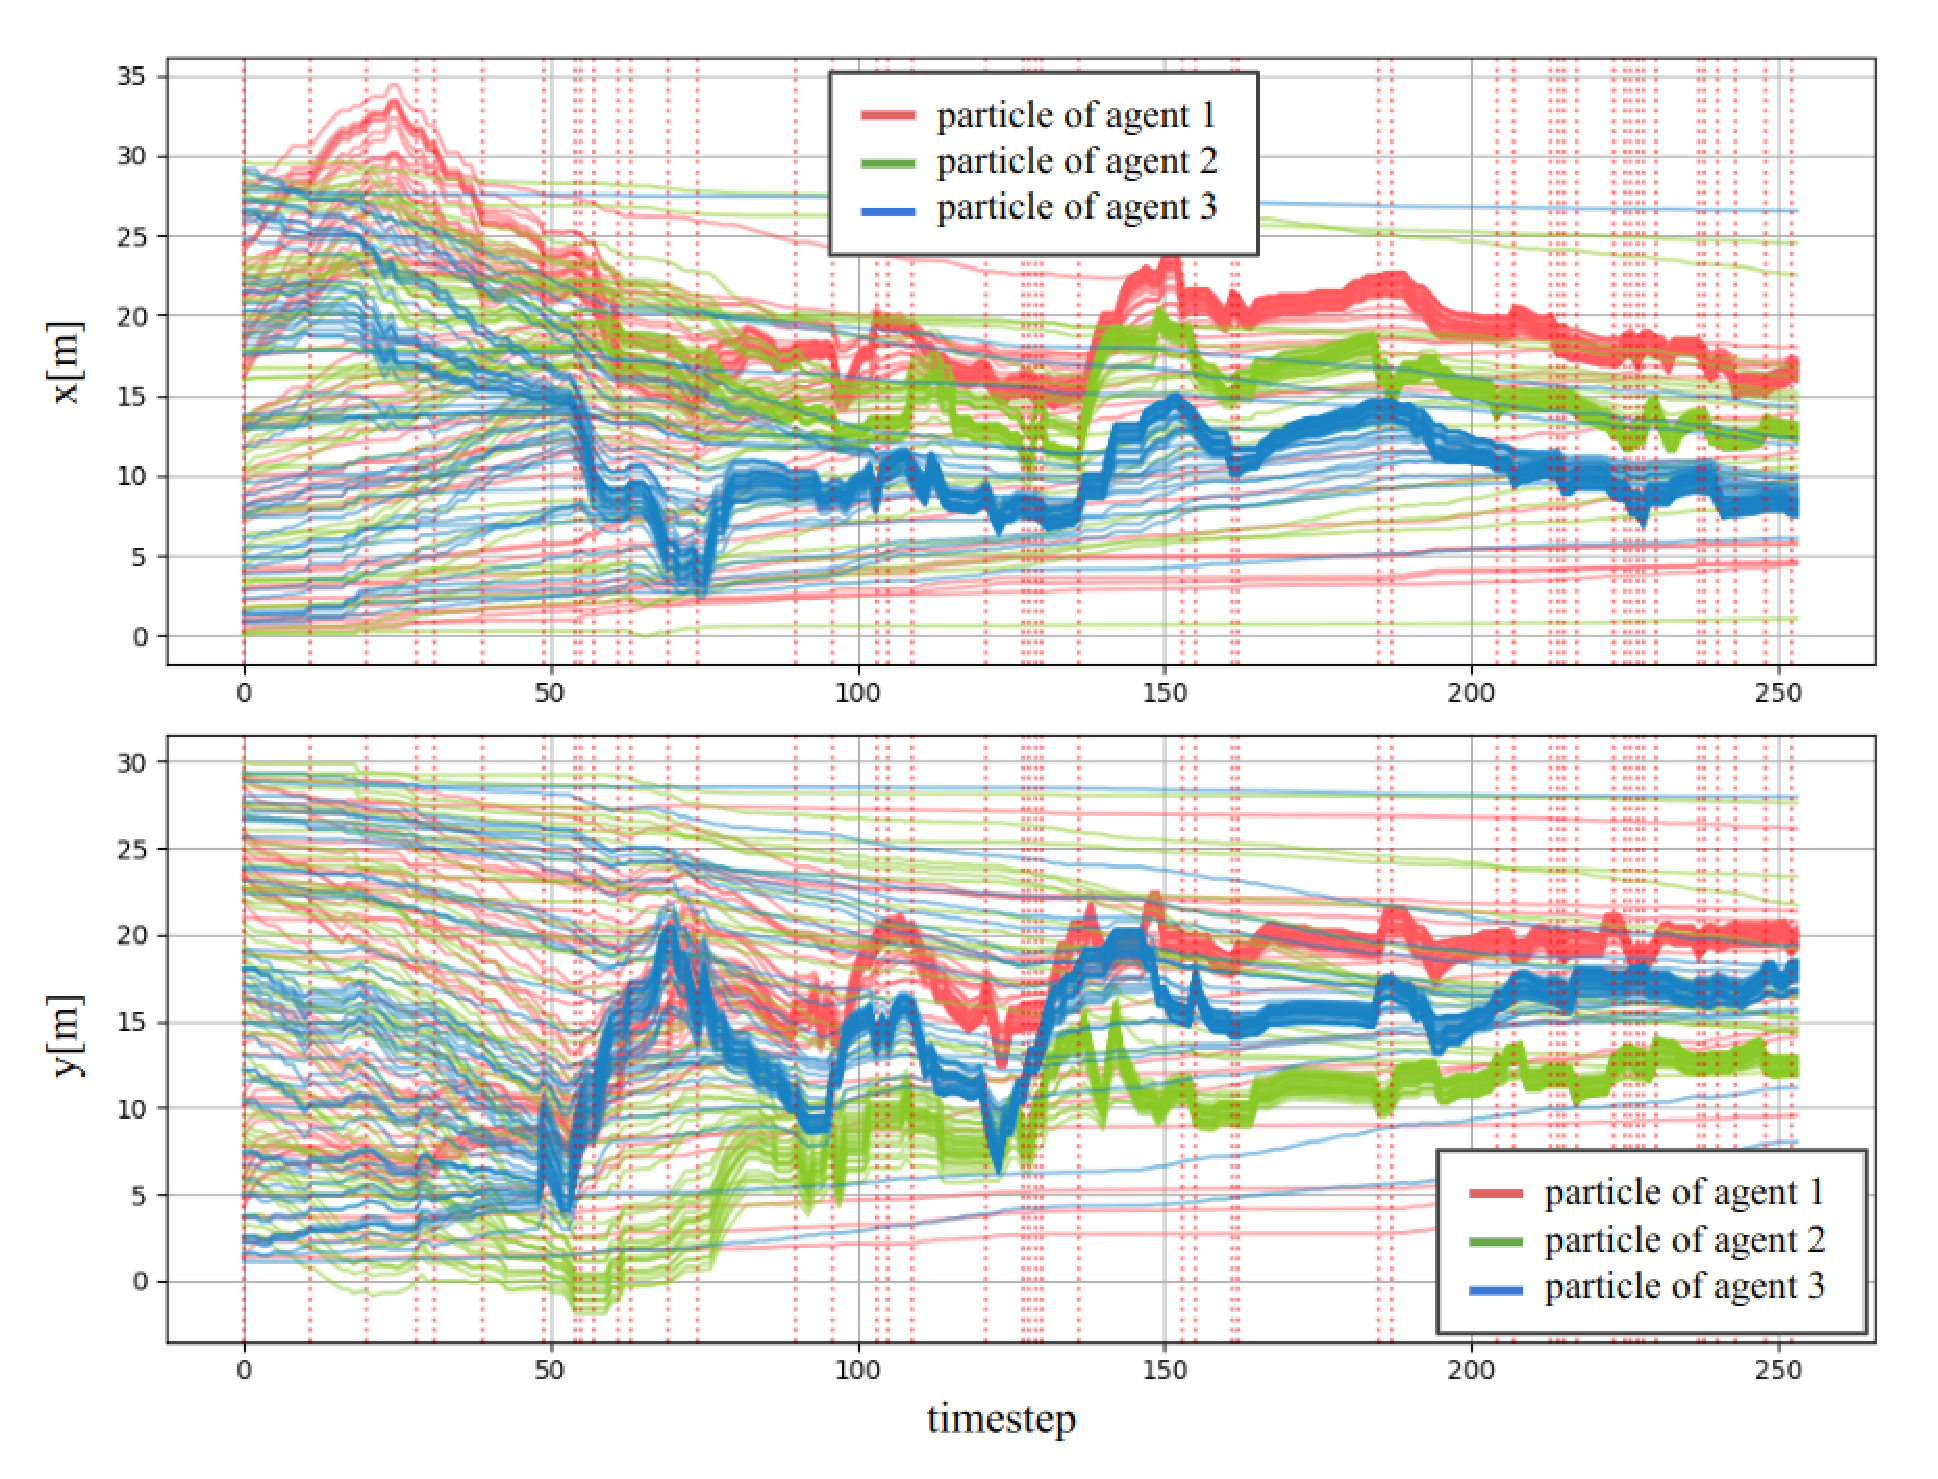
\includegraphics[width=\linewidth]{Fig/2d_plot.eps}
		\caption{Time transition of the coordinates $p_{i,r}$ of all particles in the two-dimensional cooperative self-localization simulation, shown separately for x-coordinates and y-coordinates.
    Each line plotted represents the coordinates of an agent's particles.
    The red vertical dotted lines indicate the steps where outliers were generated.}
		\label{fig:plot_1}
	\end{center}
	\vspace{-2mm}
\end{figure}

\subsection{Three-dimensional case}

As a validation of the proposed method in SE(3), we conducted a simulation of a 3D cooperative self-localization scenario.
Validation in three-dimensional space is important for reproducing environments closer to the actual operating environments of UAVs.
In particular, state estimation on the special Euclidean group SE(3), which includes rotation matrices, requires handling both pose and position simultaneously, making it computationally and theoretically more complex than the two-dimensional case.
The simulation conditions are shown in Table \ref{tb:sim2}.

\begin{table}[h]
\caption{Simulation Conditions}
  \centering
  \begin{tabular}{l|c} \hline
    Item & Value  \\ \hline
    Number of agents & 3  \\
    Number of particles per agent & 50  \\ 
    Number of time steps & 250 \\
    Total number of matches & 250 \\ 
    Number of incorrect matches & 48 \\
    Proportion of outliers & $\simeq$ 0.2 \\ \hline
  \end{tabular}
  \label{tb:sim2}
\end{table}

The simulation setup is similar to the 2D case, assuming true agent positions and that relative values between random agent pairs are obtained at each step, recreating an environment where outliers are mixed in at a certain proportion.
In the 3D simulation, the true agent positions were set as:
\begin{equation}
  \begin{aligned}
  x_i = 
  \begin{pmatrix}
    {\mathbf{I}} & {\mathbf{t}}_i \\
    {\mathbf{0}}^T & 1
  \end{pmatrix}, {\mathbf{t}}_1 = \begin{bmatrix} 0 \\ 0 \\ 0 \end{bmatrix}, {\mathbf{t}}_2 = \begin{bmatrix} 2 \\ 0 \\ 0 \end{bmatrix}, {\mathbf{t}}_3 = \begin{bmatrix} 0 \\ 2 \\ 0 \end{bmatrix}
  \end{aligned}
\end{equation}
and estimation was performed.

In the three-dimensional simulation, as shown in Fig. \ref{fig:3d_simulation}, similar to the two-dimensional case, we observed the process of each agent gradually converging from the initial state to accurate position and pose estimation. A particularly noteworthy point is that the gradient calculation on SE(3) functioned accurately, and appropriate convergence was observed in both the rotation and translation components. Additionally, even in an environment with outliers, the consensus algorithm using ADMM proposed in this method functioned effectively, confirming that all agents converged to a consistent state estimation.

Compared to the two-dimensional case, the computational cost increased in the three-dimensional simulation, but thanks to the benefits of parallel processing on the GPU, results could be obtained within a practical computation time.

\begin{figure}[t]
	\begin{center}
		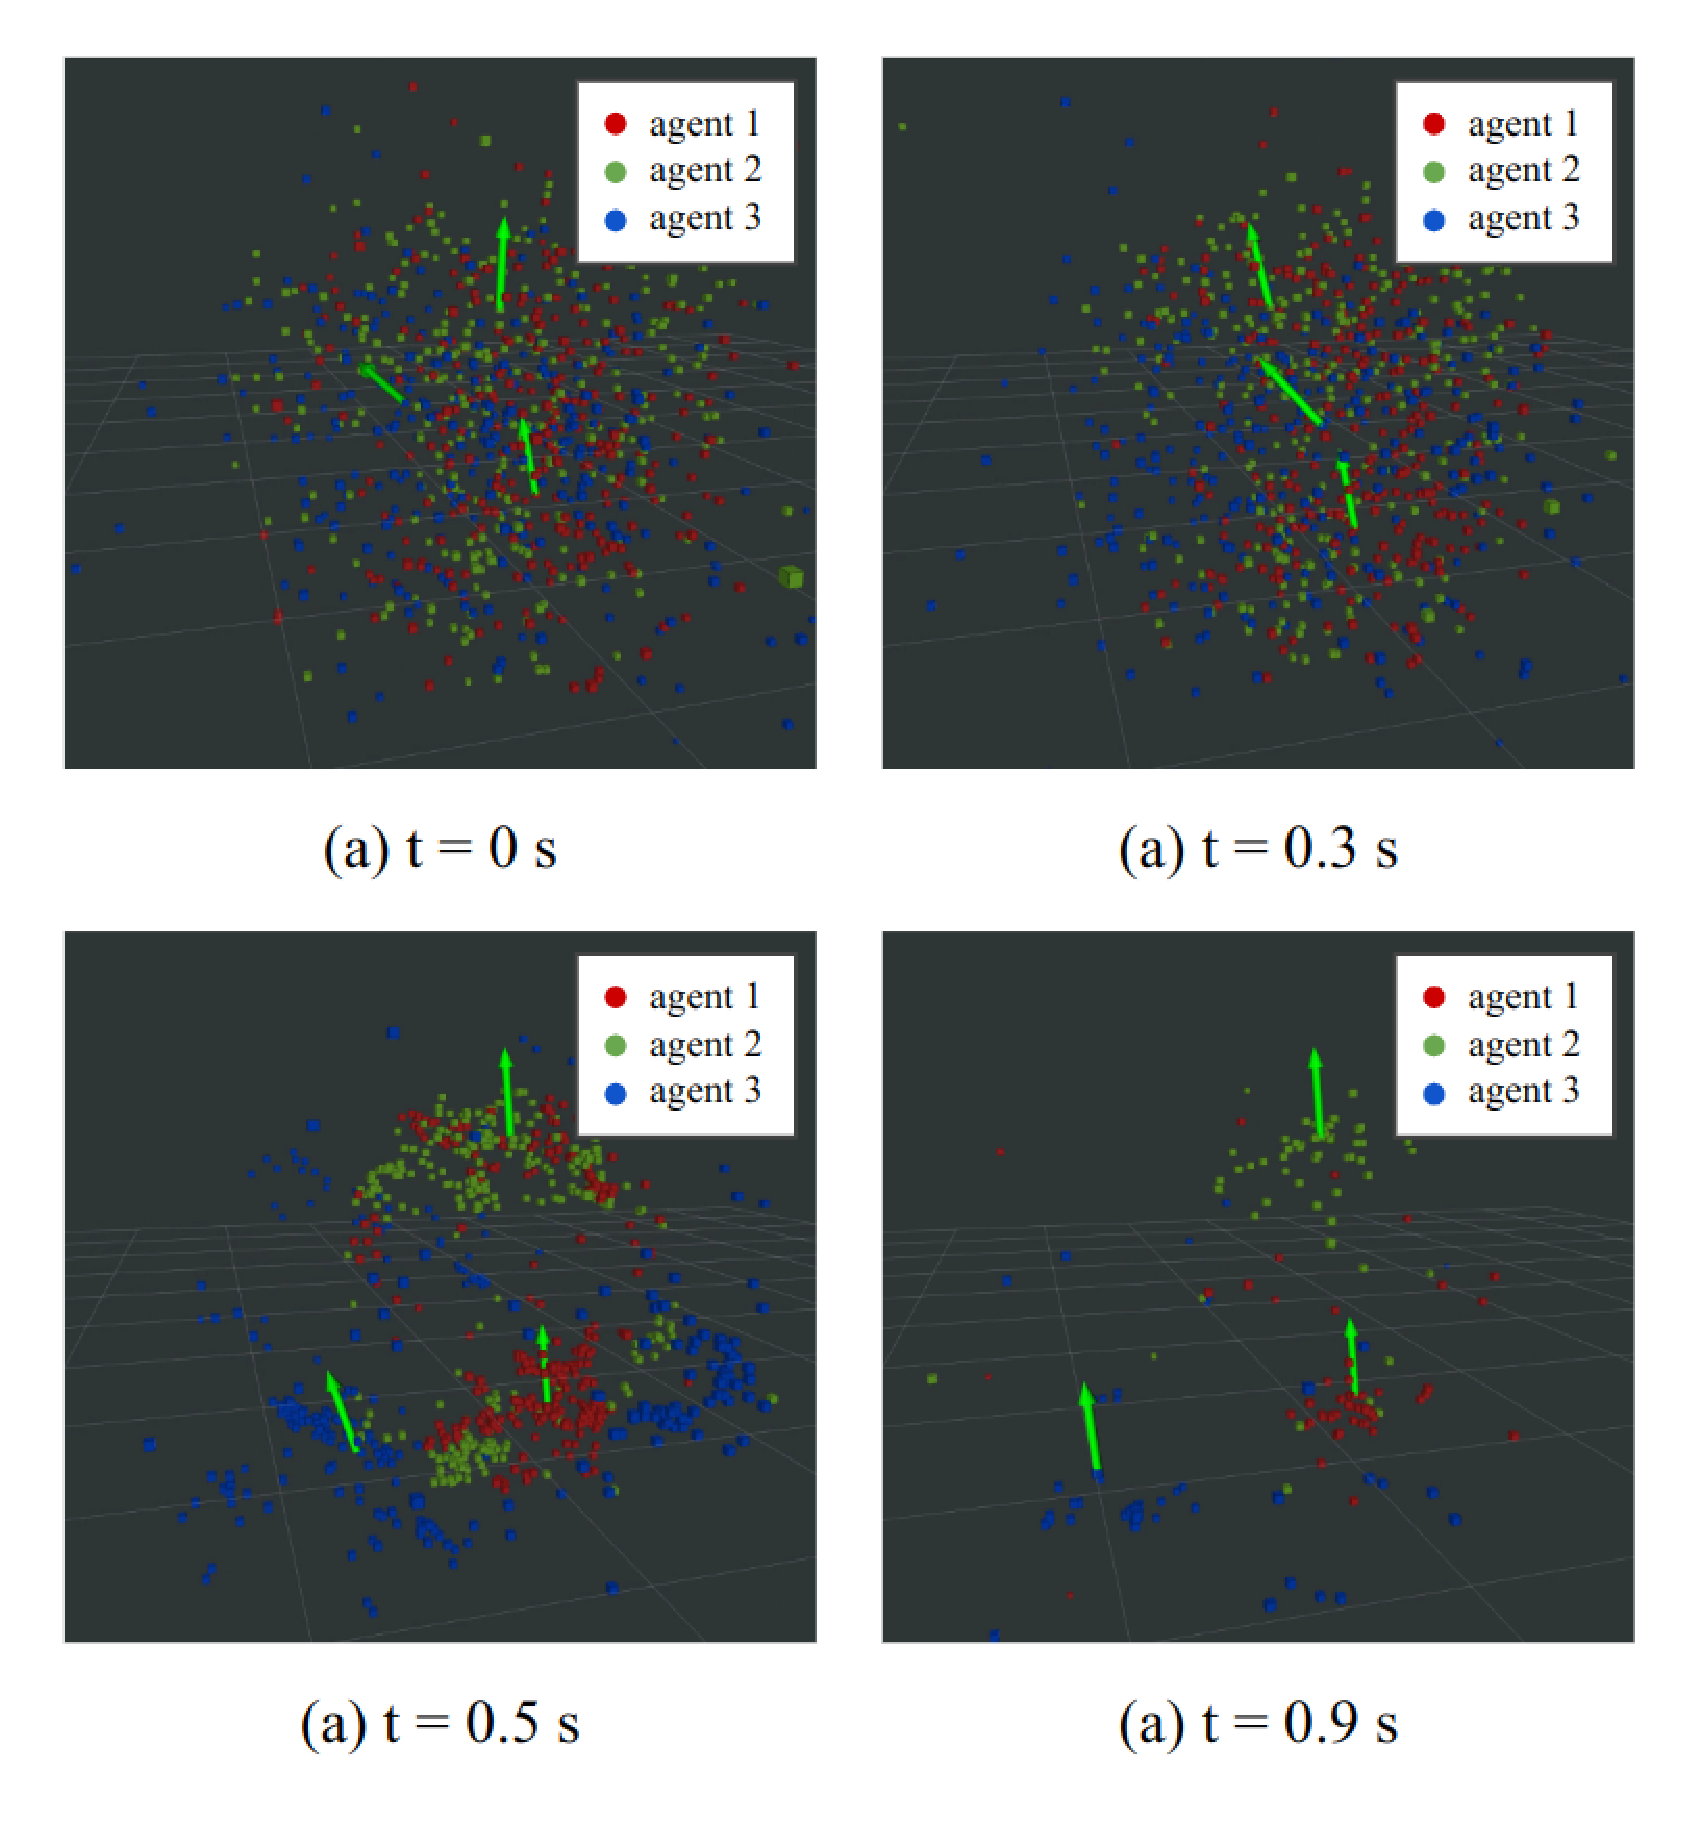
\includegraphics[width=\linewidth]{Fig/3d_simulation.eps}
		\caption{Three-dimensional cooperative self-localization simulation with an outlier ratio of 0.2. The images show the state at (a) 0s, (b) 0.3s, (c) 0.5s, and (d) 0.9s from the start of the simulation.
    The point clouds are the coordinates $p_{i,r}$ of each agent's particles. The yellow-green arrows represent the self-positions estimated from each agent's point cloud.}
		\label{fig:3d_simulation}
	\end{center}
	\vspace{-2mm}
\end{figure}

\section{Extension to the Visual Inertial System}

As a partial validation for applying the proposed method to a real cooperative self-localization system, we conducted a single-agent hardware experiment using a UAV equipped with a BMI270 IMU and an Intel RealSense D435 camera.
Hardware experiments are essential for considering complex real-world elements (sensor noise, environmental uncertainties, computational delays, etc.) that are difficult to reproduce in simulations. In particular, for Visual-Inertial Systems, it is important to verify the accuracy and stability of self-localization through the integration of cameras and IMUs in a real environment.

For the prediction step, we need to calculate $P(x_{t+1}|z_t)$ in equation (\ref{eq:map}). This is an operation that predicts the state at step $t+1$ from the information up to step $t$, and in VINS, it is obtained by numerically integrating the acceleration $a_m$ and angular velocity $\omega_m$ obtained from the IMU. Numerical integration on SE(3) can be performed using a framework similar to that in the literature \cite{Forster2017}:

\begin{equation}
\begin{aligned}\label{eq:predict}
p_{k+1} &=p_{k} + v_{k}\Delta t \\
&\quad+ \int\!\!\!\int_{t\in [t_k,t_{k+1}]} \underbrace{\left \{ R_{k}(a_m-b_a-\eta_{ad})+g\right \}}_{\hat a}dt^2,\\
v_{k+1} &=v_{k} + \int_{t\in [t_k,t_{k+1}]} \hat a dt,\\
R_{k+1} &=R_{k} \otimes \exp \left( \int_{t\in [t_k,t_{k+1}]} \underbrace{(\omega_m-b_g-\eta_{gd})}_{\hat \omega} dt \right),
\end{aligned}
\end{equation}

where $p$ is position, $v$ is velocity, $R$ is the rotation matrix representing pose, $b_a, b_g$ are the biases of acceleration and angular velocity, and $\eta_{ad}, \eta_{gd}$ are white noise.
Each particle is updated by the transformation $T_{t\rightarrow t+1}\in \text{SE}(3)$ obtained through numerical integration:

\begin{equation}
\begin{aligned}\label{eq:step}
\hat x_{t+1}^i = x_{t}^i T_{t\rightarrow t+1}, \forall i,
\end{aligned}
\end{equation}

In this experiment, we focused on the following points:
\begin{itemize}
\item Robustness against outliers (incorrect visual matches) in real environments
\item Correction capability for accumulated integration errors from the IMU
\item Appropriate handling of uncertainty through multi-modal distribution representation
\item Feasibility of real-time processing
\end{itemize}

The conditions of the hardware experiment conducted are shown in Table \ref{tb:sim3}.

\begin{table}[h]
\caption{Hardware Experiment Conditions}
  \centering
  \begin{tabular}{l|c} \hline
    Item & Value  \\ \hline
    Number of agents & 1  \\
    Number of particles & 20 /agent  \\
    Proportion of outliers & 〜10\% \\
    Ground Truth & OptiTrack Flex13, Naturalpoint \\ \hline
  \end{tabular}
  \label{tb:sim3}
\end{table}

In this experiment, it was observed that the SPF based on SVGD reduced error accumulation in 6DoF state estimation and improved accuracy compared to benchmark methods (such as D2SLAM). In particular, position errors that gradually increase with long-term operation in conventional methods were effectively suppressed in the proposed method. This is thought to be because by maintaining particle diversity while utilizing gradient information, more accurate state estimation is possible without falling into local optimal solutions.

Although the full cooperative effect with multiple agents remains unverified, initial results have been obtained suggesting that the SPF-based framework proposed in this research may be useful in real environments. The results from single-agent experiments are important as basic performance indicators for extension to multiple agents, and suggest the practicality of the proposed method, particularly from the perspectives of computational efficiency and robustness.

Fig. \ref{fig:ros_demo} shows the self-localization performed using ROS.
Fig. \ref{fig:benchmark} shows the error transition between each particle and the Ground Truth in the benchmark method. From this, it can be confirmed that the proposed method estimates with higher accuracy than the benchmark method for most of the time series. This experiment verified the effectiveness of the gradient update method for particles in 6 DoF, but future research will include verification of the consensus method using multiple agents.

\begin{figure}[t]
	\begin{center}
		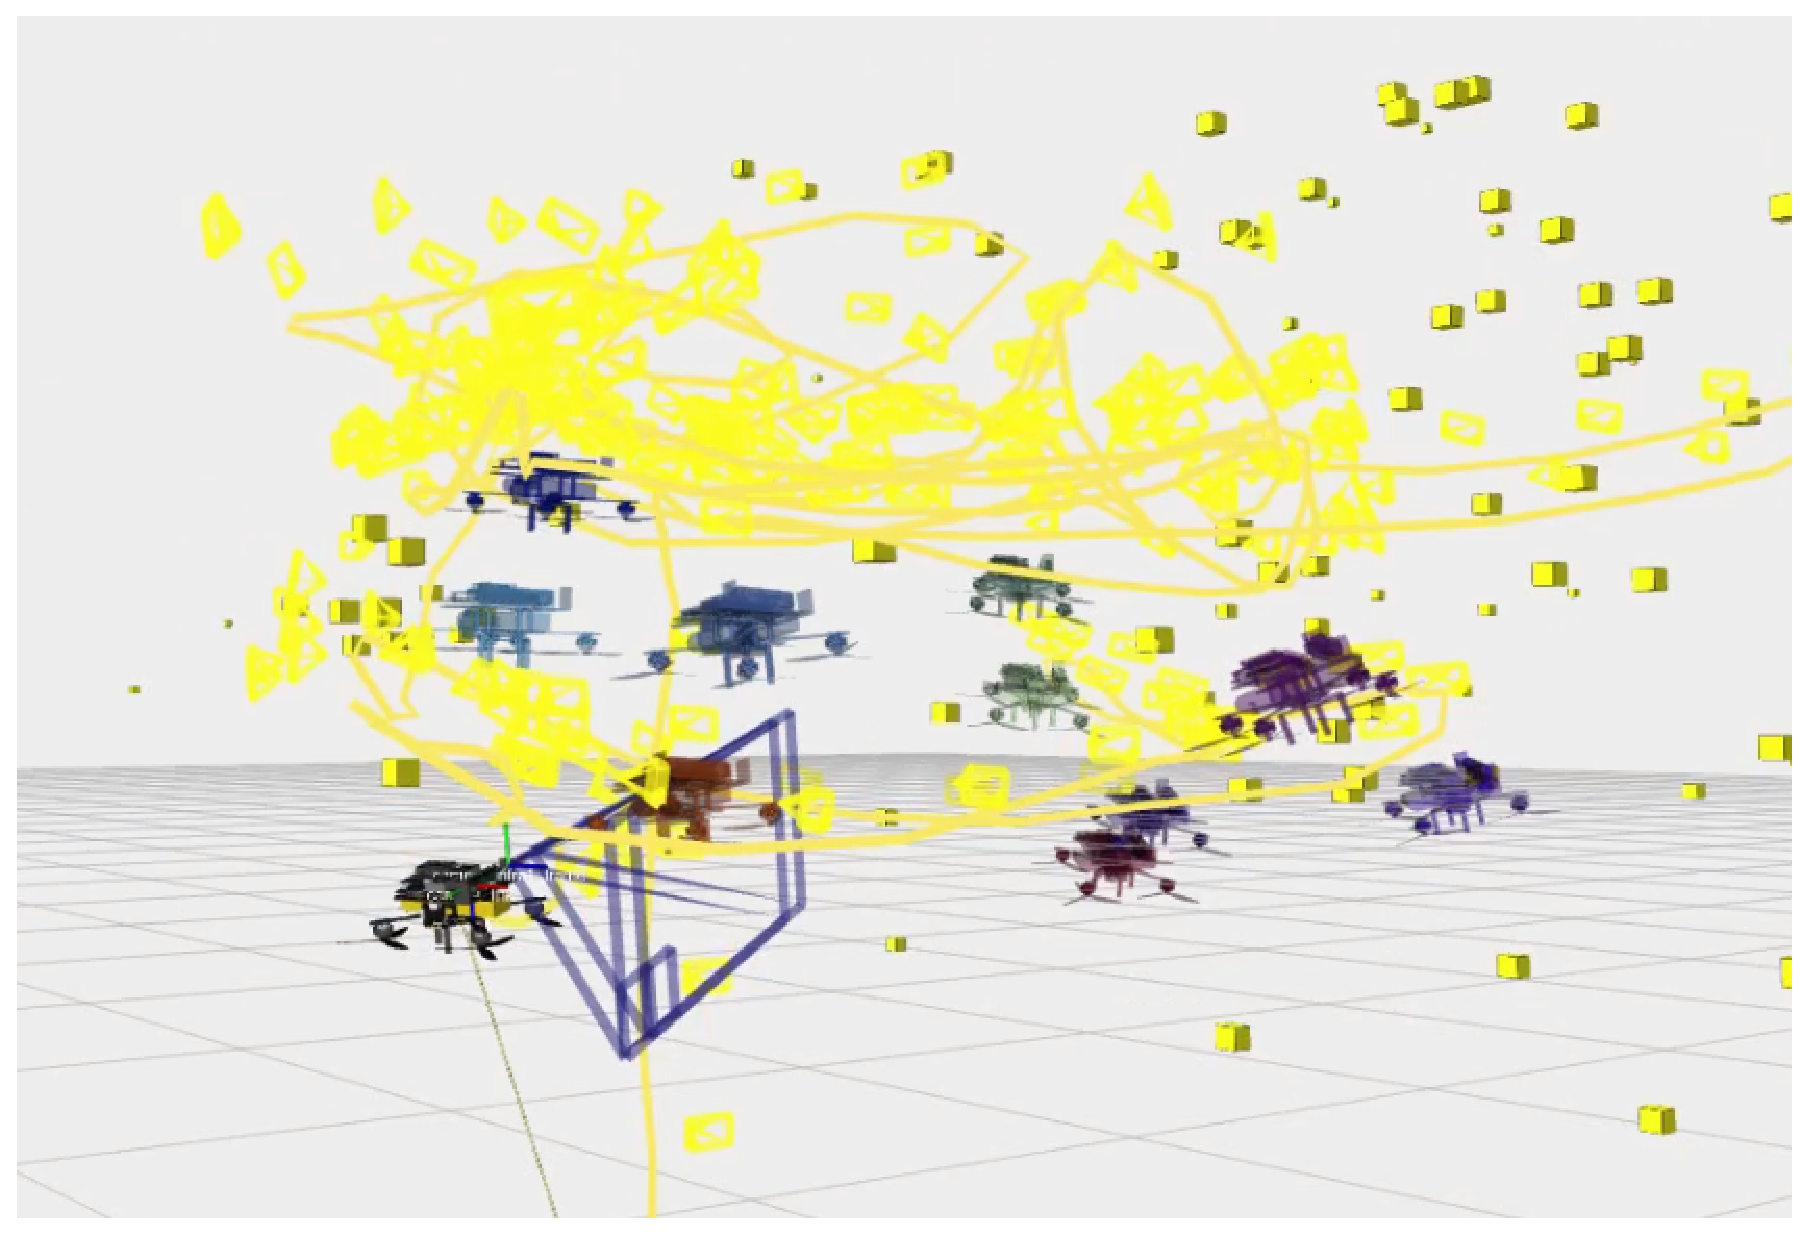
\includegraphics[width=\linewidth]{Fig/particle_filter_demo.eps}
		\caption{Verification of the proposed algorithm on ROS. The light drone 3D models represent the coordinates $p_{i,r}$ of the particles, and the dark 3D model represents the estimated position of the agent. The yellow points are feature points extracted by superpoint, and the yellow line is the estimated trajectory of the agent.}
		\label{fig:ros_demo}
	\end{center}
	\vspace{-2mm}
\end{figure}

\begin{figure}[t]
	\begin{center}
		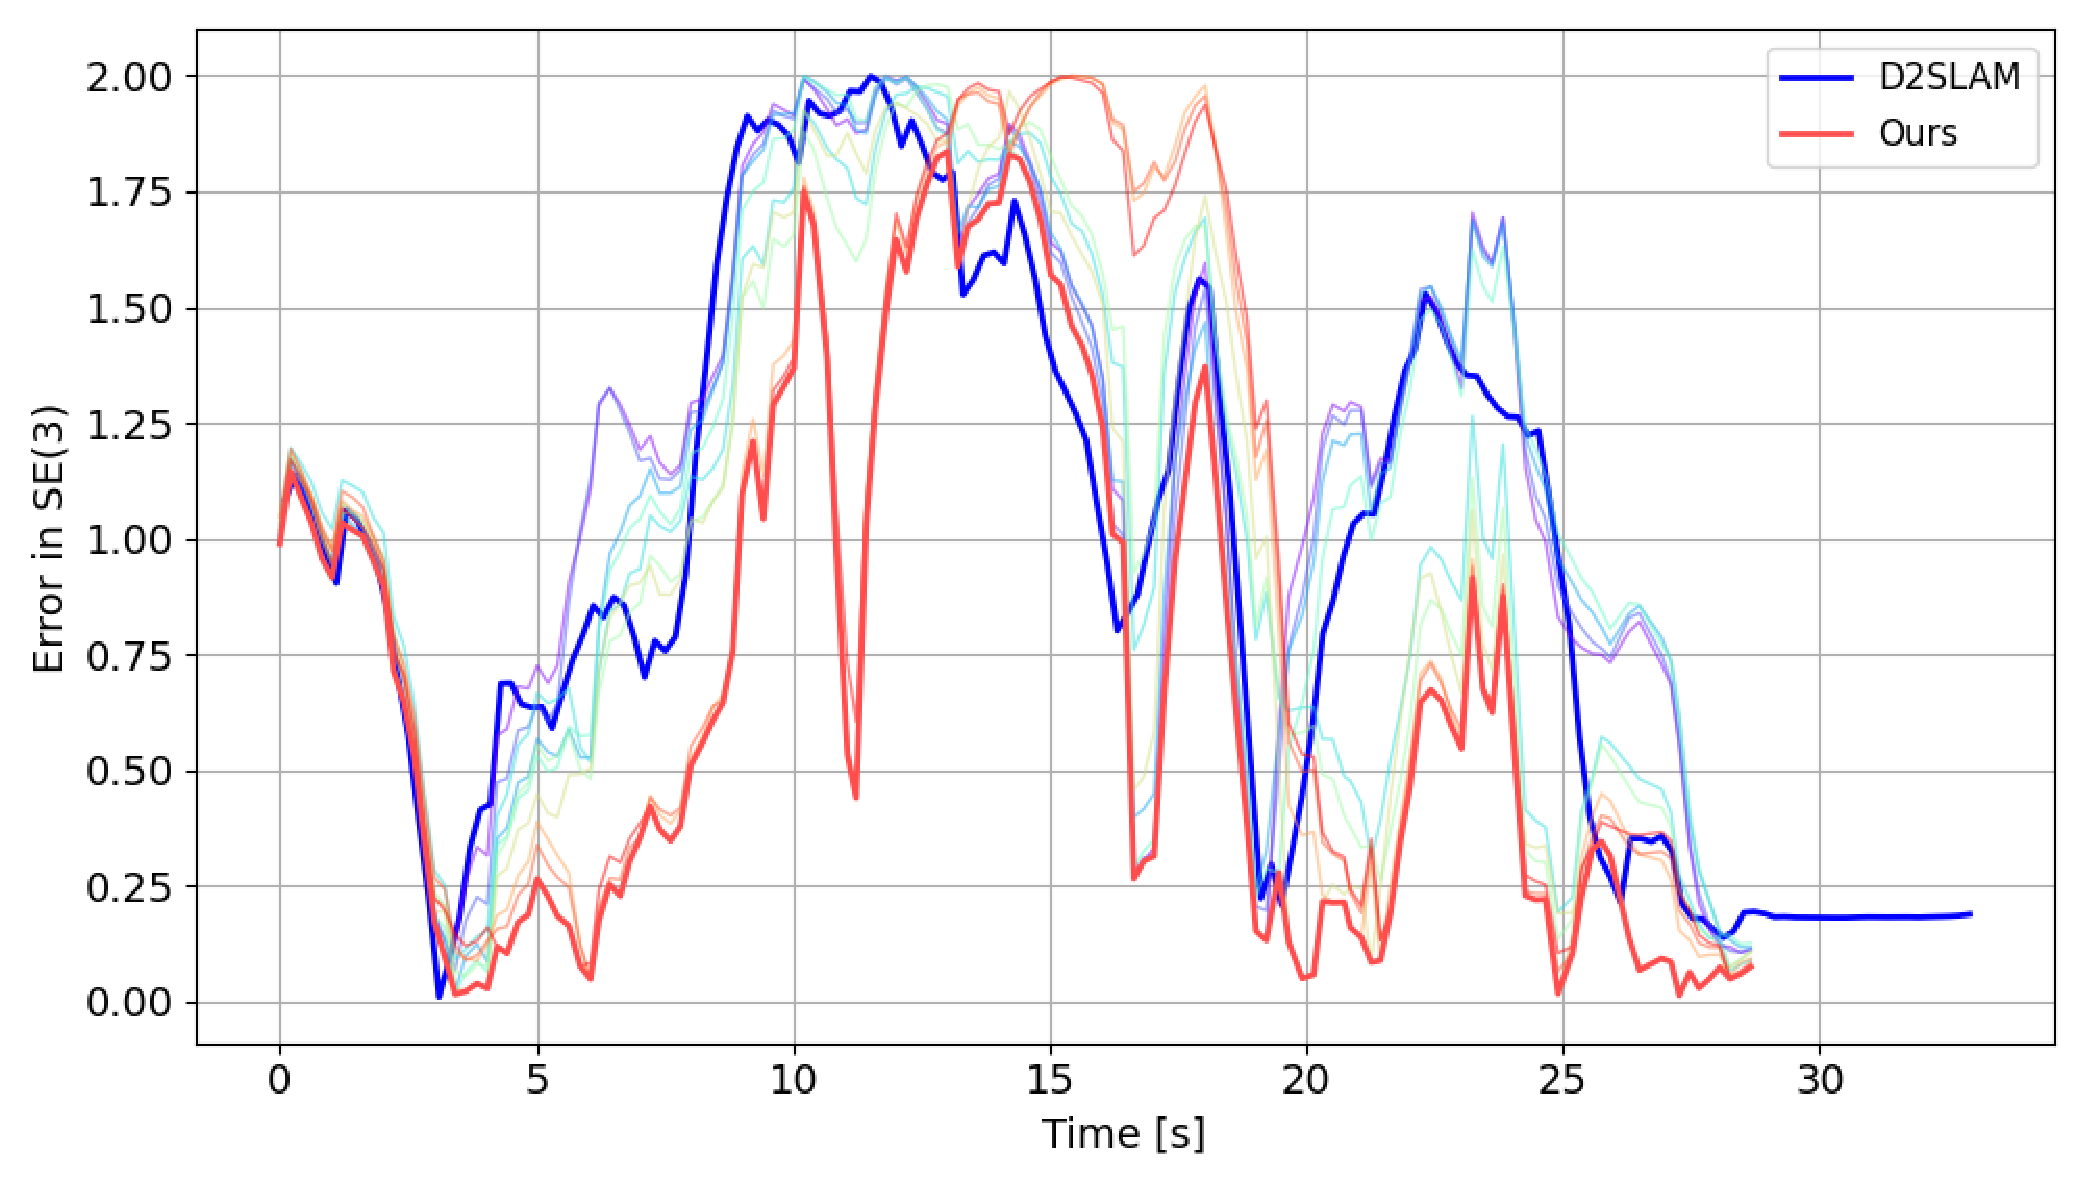
\includegraphics[width=\linewidth]{Fig/benchmark.eps}
		\caption{Benchmark of the proposed method and D2SLAM verified on ROS. The light lines represent the error time transition between each particle and the Ground Truth, and the thick orange line represents the error time transition in the estimated state of the proposed method. The thick blue line represents the error transition of D2SLAM.}
		\label{fig:benchmark}
	\end{center}
	\vspace{-2mm}
\end{figure}

\section{Conclusion}

In this paper, we proposed a new framework combining SPF and Relaxed ADMM to address the cooperative self-localization problem of UAVs in monotone wide-area environments.
In particular, we presented a theoretically consistent solution to two fundamental challenges faced by conventional cooperative self-localization methods: "the influence of outliers" and "consistent state estimation among agents."

The proposed method enables simultaneous handling of consensus constraints among multiple agents and multi-modal distributions, achieving stable position consensus in environments with outliers, which was difficult with conventional methods.
Specifically, this was achieved through three technical contributions: (1) representation and manipulation of probability distributions on the special Euclidean space SE(d), (2) introduction of a distributed optimization framework using ADMM, and (3) appropriate handling of uncertainty through particle-based representation. The combination of these significantly improved the accuracy and stability of cooperative self-localization in monotone environments.

From simulation and hardware experiment (single-agent) results, it was suggested that using SPF enables more robust and flexible self-localization than existing methods by utilizing distribution approximation and gradient information.
In particular, the fact that stable convergence was obtained even in environments with an outlier ratio of about 0.2 is an important achievement from a practical perspective. It was also confirmed that real-time processing can be realized while suppressing the increase in computational cost through parallel computation using GPUs.

In the future, we plan to further verify the effectiveness and scalability of the proposed method through large-scale experiments at the hardware level with multiple UAVs.

\appendix
\section{Proof of Theorems}

\subsection{Proof of Theorem 2 (Relaxed ADMM Algorithm for Probability Distributions)}
This proof demonstrates the derivation process of the Relaxed ADMM algorithm for solving the constrained optimization problem for probability distributions represented by equation (\ref{eq:kl_consensus_relaxed}). First, we apply the standard Relaxed ADMM framework to the probability distribution optimization problem, and then perform transformations considering the specific properties of probability distributions.

First, we construct the augmented Lagrangian for the constraint between agent $i$ and agent $j$ introduced with slack variable $y_{ij}$:

\begin{equation}
\begin{aligned}
y^+_{ij}&= \underset{y_{ij}}{\text{arg min}}\: {\mathcal{L}}_{g,\gamma}(z_{ij,i} + z_{ij,j})\\
&=  \underset{y_{ij}}{\text{arg min}}\: \langle z_{ij,i} + z_{ij,j}, y_{ij} \rangle +  \frac \gamma 2\|y_{ij}\|^2 ,
\end{aligned}
\end{equation}

where $z_{ij,i}$ and $z_{ij,j}$ are the Lagrange multipliers for agents $i$ and $j$ respectively, and $\gamma$ is the penalty parameter. Solving this minimization problem gives the update equation for $y_{ij}$. Next, we calculate the auxiliary variable $\omega_g$:

\begin{equation}
\begin{aligned}
(\omega_g)_{ij,i} &= z_{ij,i} - \gamma y^+_{ij},
\end{aligned}
\end{equation}

Using this auxiliary variable, we update the state $x_i$ of agent $i$. The augmented Lagrangian for probability distribution $P_i$ is expressed as:

\begin{equation}
\begin{aligned}
x^+_i&= \underset{x_i}{\text{arg min}}\: {\mathcal{L}}_{F,\gamma}(x_i, z_i)\\
&=  \underset{x_i}{\text{arg min}}\: D_{KL} ({P_i}_{[T]}\|{P_Q}_i) \\
& \quad - \sum_{j\in {\mathcal{E}}_i} \int_{P_i} \left\{2(\omega_g)_{ij,i} - z_{ij,i}\right\} dx_i\\
& \quad + \frac{\gamma}{2}|{\mathcal{E}}_i|\int_{P_i} dx_i^2,
\end{aligned}
\end{equation}

where $D_{KL} ({P_i}_{[T]}\|{P_Q}_i)$ is the KL divergence term, and ${\mathcal{E}}_i$ is the set of adjacent agents to agent $i$. Solving this minimization problem updates the probability distribution $P_i$.

Next, we calculate another auxiliary variable $\omega_f$:

\begin{equation}
\begin{aligned}
(\omega_f)_{ij,i} &= 2(\omega_g)_{ij,i} - z_{ij,i} - \gamma x^+_{i},
\end{aligned}
\end{equation}

Finally, we update the Lagrange multiplier $z_{ij,i}$:

\begin{equation}
\begin{aligned}
z^+_{ij,i}&=z_{ij,i}+\eta((\omega_f)_{ij,i}-(\omega_g)_{ij,i}),
\end{aligned}
\end{equation}

where $\eta$ is the step size parameter.

Organizing these update equations gives the Relaxed ADMM algorithm shown in Theorem 2. This algorithm can simultaneously optimize both the local probability distributions of each agent and the consensus constraints between agents. In particular, by using the expectation representation of probability distributions, it can be transformed into the form shown in equation (\ref{eq:prob_relaxed_admm}).

\subsection{Proof of Theorem 3 (Additional Terms as Exponential Penalties)}
This proof demonstrates how additional penalty terms act on the reference distribution in a probability distribution optimization problem. Specifically, it shows that the solution to an optimization problem including KL divergence and additional terms can be expressed as the reference distribution with exponential weights.

First, we write out the objective function in terms of $P_i$:
\begin{equation}
\begin{aligned}
{\mathcal{J}}(P_i) &= \int P_i(x_i)\log\frac{P_i(x_i)}{P_{Q_i}(x_i)}\,dx_i \\
&+ \sum_{r \in {\mathcal{E}}_i}\int P_i(x_i) z_{ir,r}(x_i)\,dx_i  \\
&+ \frac{\gamma}{2}|{\mathcal{E}}_i| \int P_i(x_i) x_i^2\, dx_i,
\end{aligned}
\end{equation}

where the first term is the KL divergence $D_{KL}(P_i \,\|\, P_{Q_i})$, and the second and third terms are additional penalty terms. Combining these terms into a single integral:

\begin{equation}
\begin{aligned}
{\mathcal{J}}(P_i) &= \int P_i(x_i)\biggl(\log P_i(x_i) - \log P_{Q_i}(x_i) \\
&\quad + \sum_{r \in {\mathcal{E}}_i} z_{ir,r}(x_i)
+ \frac{\gamma}{2}|{\mathcal{E}}_i| x_i^2 \biggr) dx_i,
\end{aligned}
\end{equation}

Next, we optimize with respect to $P_i$. Since $P_i$ is a probability distribution, there is a constraint $\int P_i(x_i)\,dx_i=1$. We use the Lagrange multiplier method to solve this constrained optimization problem. Introducing the Lagrange multiplier $\lambda$:

\begin{equation}
\begin{aligned}
&\delta_{P_i}\Bigl[\int P_i(x_i)\log P_i(x_i)\,dx_i\\
&- \int P_i(x_i)\log P_{Q_i}(x_i)\,dx_i\\
&+ \int P_i(x_i)\bigl(\sum_{r \in {\mathcal{E}}_i} z_{ir,r}(x_i)+ \frac{\gamma}{2}|{\mathcal{E}}_i|x_i^2\bigr)dx_i\\
&- \lambda \left(\int P_i(x_i)\,dx_i -1\right)\Bigr]= 0,
\end{aligned}
\end{equation}

where $\delta_{P_i}$ represents the variational derivative with respect to $P_i$. Computing this variational derivative:

\begin{equation}
\begin{aligned}
&\log P_i(x_i) + 1 - \log P_{Q_i}(x_i) \\
&+ \sum_{r \in {\mathcal{E}}_i} z_{ir,r}(x_i) 
+ \frac{\gamma}{2}|{\mathcal{E}}_i| x_i^2 - \lambda = 0,
\end{aligned}
\end{equation}

Solving for $P_i(x_i)$:

\begin{equation}
\begin{aligned}
&\log P_i(x_i) = \log P_{Q_i}(x_i) \\
&- \sum_{r \in {\mathcal{E}}_i} z_{ir,r}(x_i)
- \frac{\gamma}{2}|{\mathcal{E}}_i| x_i^2 + \lambda - 1,
\end{aligned}
\end{equation}

where $\lambda-1$ is a constant that satisfies the normalization condition of the probability distribution. Denoting this as $-\log Z$:

\begin{equation}
\begin{aligned}
&\log P_i(x_i) = \log P_{Q_i}(x_i) \\
&- \sum_{r \in {\mathcal{E}}_i} z_{ir,r}(x_i)
- \frac{\gamma}{2}|{\mathcal{E}}_i| x_i^2 - \log Z,
\end{aligned}
\end{equation}

Taking the exponential of both sides, the optimal distribution $P_i^*(x_i)$ is expressed as:

\begin{equation}
\begin{aligned}
P_i^*(x_i) = \frac{P_{Q_i}(x_i)\exp\left(- \sum_{r \in {\mathcal{E}}_i} z_{ir,r}(x_i) 
- \frac{\gamma}{2}|{\mathcal{E}}_i| x_i^2\right)}{Z},
\end{aligned}
\end{equation}

where $Z$ is the normalization constant:

\begin{equation}
\begin{aligned}
Z = \int P_{Q_i}(x_i)\exp\left(- \sum_{r \in {\mathcal{E}}_i} z_{ir,r}(x_i) 
- \frac{\gamma}{2}|{\mathcal{E}}_i| x_i^2\right) dx_i,
\end{aligned}
\end{equation}

From this result, it is clear that the additional penalty terms:

\begin{equation}
\begin{aligned}
\sum_{r \in {\mathcal{E}}_i} z_{ir,r}(x_i) \;+\; \frac{\gamma}{2}|{\mathcal{E}}_i|x_i^2,
\end{aligned}
\end{equation}

give weights to the reference distribution $P_{Q_i}(x_i)$ in the form of an exponential function. That is, these terms act as exponential penalties on the reference distribution, playing an important role in characterizing the shape of the optimal distribution.

Thus, Theorem 3 is proven.

\begin{thebibliography}{99}
\bibitem{Qin2018} T. Qin, P. Li, and S. Shen, ``VINS-Mono: A Robust and Versatile Monocular Visual-Inertial State Estimator,'' {\it IEEE Transactions on Robotics}, Vol. 34, No. 4, pp. 1004-1020, 2018.

\bibitem{Chen2021} C. Chen, H. Zhu, M. Li, and S. You, ``A Review of Visual-Inertial Simultaneous Localization and Mapping from Filtering-Based and Optimization-Based Perspectives,'' {\it Robotics}, Vol. 7, No. 3, pp. 45, 2021.

\bibitem{Zhou2018} X. Zhou, J. Zhu, H. Zhou, C. Xu, and F. Gao, ``EGO-Swarm: A Fully Autonomous and Decentralized Quadrotor Swarm System in Cluttered Environments,'' {\it IEEE International Conference on Robotics and Automation (ICRA)}, pp. 7308-7315, 2018.

\bibitem{Liu2016} Q. Liu and D. Wang, ``Stein Variational Gradient Descent: A General Purpose Bayesian Inference Algorithm,'' {\it Advances in Neural Information Processing Systems (NeurIPS)}, pp. 2378-2386, 2016.

\bibitem{Koide2021} K. Koide, J. Miura, and E. Menegatti, ``A Portable 3D LIDAR-based System for Long-term and Wide-area People Behavior Measurement,'' {\it International Journal of Advanced Robotic Systems}, Vol. 16, No. 2, pp. 1-15, 2021.

\bibitem{Bloesch2017} M. Bloesch, S. Omari, M. Hutter, and R. Siegwart, ``Robust Visual Inertial Odometry Using a Direct EKF-Based Approach,'' {\it IEEE/RSJ International Conference on Intelligent Robots and Systems (IROS)}, pp. 298-304, 2017.

\bibitem{Forster2017} C. Forster, L. Carlone, F. Dellaert, and D. Scaramuzza, ``On-Manifold Preintegration for Real-Time Visual-Inertial Odometry,'' {\it IEEE Transactions on Robotics}, Vol. 33, No. 1, pp. 1-21, 2017.

\bibitem{Xu2020} W. Xu, F. Gao, and S. Shen, ``D2SLAM: Decentralized and Distributed Collaborative Visual-Inertial SLAM System for Aerial Swarm,'' {\it IEEE Transactions on Robotics}, Vol. 36, No. 6, pp. 1864-1879, 2020.

\bibitem{Maken2021} F. P. Maken, F. Ramos, and L. Ott, ``Stein Particle Filter: A Stein Variational Gradient Descent Approach to Sequential Inference,'' {\it IEEE International Conference on Robotics and Automation (ICRA)}, pp. 14591-14597, 2021.

\bibitem{Schmuck2018} P. Schmuck and M. Chli, ``CCM-SLAM: Robust and Efficient Centralized Collaborative Monocular Simultaneous Localization and Mapping for Robotic Teams,'' {\it Journal of Field Robotics}, Vol. 36, No. 4, pp. 763-781, 2018.

\bibitem{Bastianello2020} N. Bastianello, R. Carli, L. Schenato, and M. Todescato, ``Asynchronous Distributed Optimization over Lossy Networks via Relaxed ADMM: Stability and Linear Convergence,'' {\it IEEE Transactions on Automatic Control}, Vol. 65, No. 8, pp. 3350-3365, 2020.

\bibitem{Arandjelovic2016} R. Arandjelovic, P. Gronat, A. Torii, T. Pajdla, and J. Sivic, ``NetVLAD: CNN Architecture for Weakly Supervised Place Recognition,'' {\it IEEE Conference on Computer Vision and Pattern Recognition (CVPR)}, pp. 5297-5307, 2016.

\bibitem{DeTone2018} D. DeTone, T. Malisiewicz, and A. Rabinovich, ``SuperPoint: Self-Supervised Interest Point Detection and Description,'' {\it IEEE/CVF Conference on Computer Vision and Pattern Recognition Workshops (CVPRW)}, pp. 337-349, 2018.

\bibitem{Peng2016} Z. Peng, Y. Xu, M. Yan, and W. Yin, ``ARock: An Algorithmic Framework for Asynchronous Parallel Coordinate Updates,'' {\it SIAM Journal on Scientific Computing}, Vol. 38, No. 5, pp. A2851-A2879, 2016.

\bibitem{Boyd2011} S. Boyd, N. Parikh, E. Chu, B. Pelegris, and J. Eckstein, ``Distributed Optimization and Statistical Learning via the Alternating Direction Method of Multipliers,'' {\it Foundations and Trends in Machine Learning}, Vol. 3, No. 1, pp. 1-122, 2011.

\end{thebibliography}

\end{document}
